\documentclass[sigplan, anonymous, review]{acmart}

\usepackage{booktabs} % For formal tables
\usepackage[utf8x]{inputenc}
\usepackage{ucs}
\usepackage{graphicx}
\usepackage{amsmath,amsthm}
\usepackage{amssymb}
\usepackage{url}
\usepackage{stmaryrd}
\usepackage{ifpdf}
\ifpdf
  \usepackage{hyperref}
\fi
\usepackage{float}
\usepackage{proof}

% Copyright
%\setcopyright{none}
%\setcopyright{acmcopyright}
%\setcopyright{acmlicensed}
\setcopyright{rightsretained}
%\setcopyright{usgov}
%\setcopyright{usgovmixed}
%\setcopyright{cagov}
%\setcopyright{cagovmixed}


% DOI
%\acmDOI{10.475/123_4}

% ISBN
%\acmISBN{123-4567-24-567/08/06}

%Conference
%\acmConference[HASKELL'17]{ACM Haskell Symposium}{July 2017}{El
 % Paso, Texas USA} 
\acmYear{2017}
\copyrightyear{2017}

%\acmPrice{15.00}

%\acmBadgeL[http://ctuning.org/ae/ppopp2016.html]{ae-logo}
%\acmBadgeR[http://ctuning.org/ae/ppopp2016.html]{ae-logo}


%% ODER: format ==         = "\mathrel{==}"
%% ODER: format /=         = "\neq "
%
%
\makeatletter
\@ifundefined{lhs2tex.lhs2tex.sty.read}%
  {\@namedef{lhs2tex.lhs2tex.sty.read}{}%
   \newcommand\SkipToFmtEnd{}%
   \newcommand\EndFmtInput{}%
   \long\def\SkipToFmtEnd#1\EndFmtInput{}%
  }\SkipToFmtEnd

\newcommand\ReadOnlyOnce[1]{\@ifundefined{#1}{\@namedef{#1}{}}\SkipToFmtEnd}
\usepackage{amstext}
\usepackage{amssymb}
\usepackage{stmaryrd}
\DeclareFontFamily{OT1}{cmtex}{}
\DeclareFontShape{OT1}{cmtex}{m}{n}
  {<5><6><7><8>cmtex8
   <9>cmtex9
   <10><10.95><12><14.4><17.28><20.74><24.88>cmtex10}{}
\DeclareFontShape{OT1}{cmtex}{m}{it}
  {<-> ssub * cmtt/m/it}{}
\newcommand{\texfamily}{\fontfamily{cmtex}\selectfont}
\DeclareFontShape{OT1}{cmtt}{bx}{n}
  {<5><6><7><8>cmtt8
   <9>cmbtt9
   <10><10.95><12><14.4><17.28><20.74><24.88>cmbtt10}{}
\DeclareFontShape{OT1}{cmtex}{bx}{n}
  {<-> ssub * cmtt/bx/n}{}
\newcommand{\tex}[1]{\text{\texfamily#1}}	% NEU

\newcommand{\Sp}{\hskip.33334em\relax}


\newcommand{\Conid}[1]{\mathit{#1}}
\newcommand{\Varid}[1]{\mathit{#1}}
\newcommand{\anonymous}{\kern0.06em \vbox{\hrule\@width.5em}}
\newcommand{\plus}{\mathbin{+\!\!\!+}}
\newcommand{\bind}{\mathbin{>\!\!\!>\mkern-6.7mu=}}
\newcommand{\rbind}{\mathbin{=\mkern-6.7mu<\!\!\!<}}% suggested by Neil Mitchell
\newcommand{\sequ}{\mathbin{>\!\!\!>}}
\renewcommand{\leq}{\leqslant}
\renewcommand{\geq}{\geqslant}
\usepackage{polytable}

%mathindent has to be defined
\@ifundefined{mathindent}%
  {\newdimen\mathindent\mathindent\leftmargini}%
  {}%

\def\resethooks{%
  \global\let\SaveRestoreHook\empty
  \global\let\ColumnHook\empty}
\newcommand*{\savecolumns}[1][default]%
  {\g@addto@macro\SaveRestoreHook{\savecolumns[#1]}}
\newcommand*{\restorecolumns}[1][default]%
  {\g@addto@macro\SaveRestoreHook{\restorecolumns[#1]}}
\newcommand*{\aligncolumn}[2]%
  {\g@addto@macro\ColumnHook{\column{#1}{#2}}}

\resethooks

\newcommand{\onelinecommentchars}{\quad-{}- }
\newcommand{\commentbeginchars}{\enskip\{-}
\newcommand{\commentendchars}{-\}\enskip}

\newcommand{\visiblecomments}{%
  \let\onelinecomment=\onelinecommentchars
  \let\commentbegin=\commentbeginchars
  \let\commentend=\commentendchars}

\newcommand{\invisiblecomments}{%
  \let\onelinecomment=\empty
  \let\commentbegin=\empty
  \let\commentend=\empty}

\visiblecomments

\newlength{\blanklineskip}
\setlength{\blanklineskip}{0.66084ex}

\newcommand{\hsindent}[1]{\quad}% default is fixed indentation
\let\hspre\empty
\let\hspost\empty
\newcommand{\NB}{\textbf{NB}}
\newcommand{\Todo}[1]{$\langle$\textbf{To do:}~#1$\rangle$}

\EndFmtInput
\makeatother
%
%
%
%
%
%
% This package provides two environments suitable to take the place
% of hscode, called "plainhscode" and "arrayhscode". 
%
% The plain environment surrounds each code block by vertical space,
% and it uses \abovedisplayskip and \belowdisplayskip to get spacing
% similar to formulas. Note that if these dimensions are changed,
% the spacing around displayed math formulas changes as well.
% All code is indented using \leftskip.
%
% Changed 19.08.2004 to reflect changes in colorcode. Should work with
% CodeGroup.sty.
%
\ReadOnlyOnce{polycode.fmt}%
\makeatletter

\newcommand{\hsnewpar}[1]%
  {{\parskip=0pt\parindent=0pt\par\vskip #1\noindent}}

% can be used, for instance, to redefine the code size, by setting the
% command to \small or something alike
\newcommand{\hscodestyle}{}

% The command \sethscode can be used to switch the code formatting
% behaviour by mapping the hscode environment in the subst directive
% to a new LaTeX environment.

\newcommand{\sethscode}[1]%
  {\expandafter\let\expandafter\hscode\csname #1\endcsname
   \expandafter\let\expandafter\endhscode\csname end#1\endcsname}

% "compatibility" mode restores the non-polycode.fmt layout.

\newenvironment{compathscode}%
  {\par\noindent
   \advance\leftskip\mathindent
   \hscodestyle
   \let\\=\@normalcr
   \let\hspre\(\let\hspost\)%
   \pboxed}%
  {\endpboxed\)%
   \par\noindent
   \ignorespacesafterend}

\newcommand{\compaths}{\sethscode{compathscode}}

% "plain" mode is the proposed default.
% It should now work with \centering.
% This required some changes. The old version
% is still available for reference as oldplainhscode.

\newenvironment{plainhscode}%
  {\hsnewpar\abovedisplayskip
   \advance\leftskip\mathindent
   \hscodestyle
   \let\hspre\(\let\hspost\)%
   \pboxed}%
  {\endpboxed%
   \hsnewpar\belowdisplayskip
   \ignorespacesafterend}

\newenvironment{oldplainhscode}%
  {\hsnewpar\abovedisplayskip
   \advance\leftskip\mathindent
   \hscodestyle
   \let\\=\@normalcr
   \(\pboxed}%
  {\endpboxed\)%
   \hsnewpar\belowdisplayskip
   \ignorespacesafterend}

% Here, we make plainhscode the default environment.

\newcommand{\plainhs}{\sethscode{plainhscode}}
\newcommand{\oldplainhs}{\sethscode{oldplainhscode}}
\plainhs

% The arrayhscode is like plain, but makes use of polytable's
% parray environment which disallows page breaks in code blocks.

\newenvironment{arrayhscode}%
  {\hsnewpar\abovedisplayskip
   \advance\leftskip\mathindent
   \hscodestyle
   \let\\=\@normalcr
   \(\parray}%
  {\endparray\)%
   \hsnewpar\belowdisplayskip
   \ignorespacesafterend}

\newcommand{\arrayhs}{\sethscode{arrayhscode}}

% The mathhscode environment also makes use of polytable's parray 
% environment. It is supposed to be used only inside math mode 
% (I used it to typeset the type rules in my thesis).

\newenvironment{mathhscode}%
  {\parray}{\endparray}

\newcommand{\mathhs}{\sethscode{mathhscode}}

% texths is similar to mathhs, but works in text mode.

\newenvironment{texthscode}%
  {\(\parray}{\endparray\)}

\newcommand{\texths}{\sethscode{texthscode}}

% The framed environment places code in a framed box.

\def\codeframewidth{\arrayrulewidth}
\RequirePackage{calc}

\newenvironment{framedhscode}%
  {\parskip=\abovedisplayskip\par\noindent
   \hscodestyle
   \arrayrulewidth=\codeframewidth
   \tabular{@{}|p{\linewidth-2\arraycolsep-2\arrayrulewidth-2pt}|@{}}%
   \hline\framedhslinecorrect\\{-1.5ex}%
   \let\endoflinesave=\\
   \let\\=\@normalcr
   \(\pboxed}%
  {\endpboxed\)%
   \framedhslinecorrect\endoflinesave{.5ex}\hline
   \endtabular
   \parskip=\belowdisplayskip\par\noindent
   \ignorespacesafterend}

\newcommand{\framedhslinecorrect}[2]%
  {#1[#2]}

\newcommand{\framedhs}{\sethscode{framedhscode}}

% The inlinehscode environment is an experimental environment
% that can be used to typeset displayed code inline.

\newenvironment{inlinehscode}%
  {\(\def\column##1##2{}%
   \let\>\undefined\let\<\undefined\let\\\undefined
   \newcommand\>[1][]{}\newcommand\<[1][]{}\newcommand\\[1][]{}%
   \def\fromto##1##2##3{##3}%
   \def\nextline{}}{\) }%

\newcommand{\inlinehs}{\sethscode{inlinehscode}}

% The joincode environment is a separate environment that
% can be used to surround and thereby connect multiple code
% blocks.

\newenvironment{joincode}%
  {\let\orighscode=\hscode
   \let\origendhscode=\endhscode
   \def\endhscode{\def\hscode{\endgroup\def\@currenvir{hscode}\\}\begingroup}
   %\let\SaveRestoreHook=\empty
   %\let\ColumnHook=\empty
   %\let\resethooks=\empty
   \orighscode\def\hscode{\endgroup\def\@currenvir{hscode}}}%
  {\origendhscode
   \global\let\hscode=\orighscode
   \global\let\endhscode=\origendhscode}%

\makeatother
\EndFmtInput
%

\DeclareMathAlphabet{\mathkw}{OT1}{cmss}{bx}{n}


\newcommand{\EvalCtxTran}[1]{\ensuremath{\mathbb{T}[#1]}}
\newcommand{\EvalCtxProc}[1]{\ensuremath{\mathbb{P}[#1]}}

\newtheorem{Lemma}{Lemma}
\newtheorem{Theorem}{Theorem}
\theoremstyle{definition}
\newtheorem{Example}{Example}


\usepackage{color}
\newcommand{\redFG}[1]{\textcolor[rgb]{0.6,0,0}{#1}}
\newcommand{\greenFG}[1]{\textcolor[rgb]{0,0.4,0}{#1}}
\newcommand{\blueFG}[1]{\textcolor[rgb]{0,0,0.8}{#1}}
\newcommand{\orangeFG}[1]{\textcolor[rgb]{0.8,0.4,0}{#1}}
\newcommand{\purpleFG}[1]{\textcolor[rgb]{0.4,0,0.4}{#1}}
\newcommand{\yellowFG}[1]{\textcolor{yellow}{#1}}
\newcommand{\brownFG}[1]{\textcolor[rgb]{0.5,0.2,0.2}{#1}}
\newcommand{\blackFG}[1]{\textcolor[rgb]{0,0,0}{#1}}
\newcommand{\whiteFG}[1]{\textcolor[rgb]{1,1,1}{#1}}
\newcommand{\yellowBG}[1]{\colorbox[rgb]{1,1,0.2}{#1}}
\newcommand{\brownBG}[1]{\colorbox[rgb]{1.0,0.7,0.4}{#1}}

\newcommand{\ColourStuff}{
  \newcommand{\red}{\redFG}
  \newcommand{\green}{\greenFG}
  \newcommand{\blue}{\blueFG}
  \newcommand{\orange}{\orangeFG}
  \newcommand{\purple}{\purpleFG}
  \newcommand{\yellow}{\yellowFG}
  \newcommand{\brown}{\brownFG}
  \newcommand{\black}{\blackFG}
  \newcommand{\white}{\whiteFG}
}

\newcommand{\MonochromeStuff}{
  \newcommand{\red}{\blackFG}
  \newcommand{\green}{\blackFG}
  \newcommand{\blue}{\blackFG}
  \newcommand{\orange}{\blackFG}
  \newcommand{\purple}{\blackFG}
  \newcommand{\yellow}{\blackFG}
  \newcommand{\brown}{\blackFG}
  \newcommand{\black}{\blackFG}
  \newcommand{\white}{\blackFG}
}

\ColourStuff

\newcommand{\D}[1]{\blue{\mathsf{#1}}}
\newcommand{\C}[1]{\red{\mathsf{#1}}}
\newcommand{\F}[1]{\green{\mathsf{#1}}}
\newcommand{\V}[1]{\purple{\mathit{#1}}}


\newcommand{\TStep}[9]{\ensuremath{\langle  #2, #3, #4 \rangle
    \mapsto_{T_{#5}} \langle  #7, #8, #9 \rangle}}


\begin{document}


\title{Certified Bit-Coded Regular Expression Parsing}

\author{Rodrigo Ribeiro}
\affiliation{%
  \institution{Universidade Federal de Ouro Preto}
%  \streetaddress{P.O. Box 1212}
  \city{Ouro Preto} 
  \state{Minas Gerais --- Brazil} 
%  \postcode{43017-6221}
}
\email{rodrigo\text{\tt decsi\char46{}ufop\char46{}br\char125{}~~\char92{}author\char123{}André~Du~Bois\char125{}~\char92{}affiliation\char123{}\char37{}~~~\char92{}institution\char123{}Universidade~Federal~de~Pelotas\char125{}~\char37{}~~\char92{}streetaddress\char123{}P\char46{}O\char46{}~Box~1212\char125{}~~~\char92{}city\char123{}Pelotas\char125{}~~~~\char92{}state\char123{}Rio~Grande~do~Sul~\char45{}\char45{}\char45{}~Brazil\char125{}~~\char37{}~~\char92{}postcode\char123{}43017\char45{}6221\char125{}~\char125{}~\char92{}email\char123{}dubois}inf.ufpel.br}

\begin{abstract}
We describe the formalization of a regular expression (RE) parsing
algorithm that produces a bit representation of its parse tree
in the dependently typed language Agda. The algorithm computes
bit-codes using Brzozowski derivatives and we prove that 
produced codes are equivalent to parse trees ensuring the 
soundness and completeness w.r.t an inductive RE semantics.
We include the certified algorithm in a tool, developed by us,
for regular expression based search in the style of the well 
known GNU grep. Practical experiments conducted with this tool 
are reported.
\end{abstract}
%
% The code below should be generated by the tool at
% http://dl.acm.org/ccs.cfm
% Please copy and paste the code instead of the example below. 
%
\begin{CCSXML}\begin{hscode}\SaveRestoreHook
\column{B}{@{}>{\hspre}l<{\hspost}@{}}%
\column{E}{@{}>{\hspre}l<{\hspost}@{}}%
\>[B]{}\V{ccs2012>}{}\<[E]%
\ColumnHook
\end{hscode}\resethooks
 <concept>
  <concept_id>10010520.10010553.10010562</concept_id>
  <concept_desc>Computer systems organization~Embedded systems</concept_desc>
  <concept_significance>500</concept_significance>
 </concept>
 <concept>
  <concept_id>10010520.10010575.10010755</concept_id>
  <concept_desc>Computer systems organization~Redundancy</concept_desc>
  <concept_significance>300</concept_significance>
 </concept>
 <concept>
  <concept_id>10010520.10010553.10010554</concept_id>
  <concept_desc>Computer systems organization~Robotics</concept_desc>
  <concept_significance>100</concept_significance>
 </concept>
 <concept>
  <concept_id>10003033.10003083.10003095</concept_id>
  <concept_desc>Networks~Network reliability</concept_desc>
  <concept_significance>100</concept_significance>
 </concept>\begin{hscode}\SaveRestoreHook
\column{B}{@{}>{\hspre}l<{\hspost}@{}}%
\column{E}{@{}>{\hspre}l<{\hspost}@{}}%
\>[B]{}\V{/ccs2012>}{}\<[E]%
\ColumnHook
\end{hscode}\resethooks
\end{CCSXML}

\ccsdesc[500]{Computer systems organization~Embedded systems}
\ccsdesc[300]{Computer systems organization~Redundancy}
\ccsdesc{Computer systems organization~Robotics}
\ccsdesc[100]{Networks~Network reliability}

% We no longer use \terms command
%\terms{Theory}

\keywords{Certified algorithms, regular expressions, bit-codes, dependent types}

\maketitle

\section{Introduction}\label{sec:intro}

Parsing is one of the most studied problems in computer science. 
It involves the process of checking if a string of symbols conforms to
a given set of rules. Usually, parsing is preceded by the 
specification of rules in a formalism (e.g. a grammar) and, also, either the
construction of data that makes evident which rules have been used to
conclude that the string of symbols can be obtained from it or, otherwise,
an indication of an error that represents the
fact that the string of symbols cannot be generated.

In this work we are interested in the parsing problem for regular
languages (RLs)~\cite{Hopcroft2000}, i.e.~languages that can be
recognized by (non-)deterministic finite automata and equivalent
formalisms. Regular expressions (REs) are an algebraic and compact way
of specifying RLs that are extensively used in lexical analyser
generators~\cite{Lesk1990} and string search utilities~\cite{Grep}.
Since such tools are widely used and parsing is pervasive in
computing, there is a growing interest on certified parsing
algorithms~\cite{FirsovU13,FirsovU14,Danielsson2010}.  
This interest is motivated by the recent development of dependently typed
languages. Such languages are powerful enough to express algorithmic
properties as types, that are automatically checked by a compiler.

In a previous work by one the authors~\cite{Lopes2016}, we described
the formalization of an algorithm for parsing RE's based on 
derivatives. RE derivatives were introduced by
Brzozowski~\cite{Brzozowski1964} as an alternative method to compute a
finite state machine that is equivalent to a given RE and to perform
RE-based parsing. Owens et. al~\cite{Owens2009} reintroduce this concept,
since ``derivatives have been lost in the sands of time'' until his work on
functional encoding of RE derivatives have renewed interest on its use
for parsing~\cite{Might2011,Fischer2010}. 

Nielsen et. al.~\cite{Nielsen2011} introduce algorithms to build compact representation of
RE parse trees as a sequence of bits, without explicitly constructing the parse tree first
and describe algorithms that simulate a finite state machine that output the required bit list. 
Sulzmann et. al.~\cite{SulzmannL14} designed a RE derivative-based algorithm
that incrementally builds a list of bits instead of a tree as parsing result. In both works
no machine checked proof was provided and some results claimed had counter-examples
found~\cite{AusafDU16}. This work aims to fill this gap. We provide fully 
certified proofs of Sulzmann et. al. derivative based parsing algorithm that 
produces a bit sequence equivalent to traditional parse trees and we use it 
in a RE based search tool that has been developed by us, using the dependently typed language
Agda~\cite{Norell2009}.

More specifically, our contributions are:
\begin{itemize}
  \item A formalization of bit-codes for RE parse trees, as presented in~\cite{Nielsen2011},
        and machine checkable proof ofs their properties.
  \item A formalization of bit-annotated regular expressions (BRE), its semantics 
        and its soundness and completeness theorems w.r.t. standard RE semantics. 
        We also relate produced bit sequences and RE semantics proving how they 
        are related to each other.
  \item A formalization of Brzozowski derivatives for BRE and its soundness and
        completeness theorem w.r.t to BRE semantics.
  \item We build certified decision procedures for matching prefixes and subtrings
        of BRE.
\end{itemize}

The rest of this paper is organized as follows. Section~\ref{sec:agda}
presents a brief introduction to Agda. Section~\ref{sec:regexp}
describes the encoding of REs, its parse trees and their representation as 
bit-codes. In Section~\ref{sec:bitregex} we present bit-annotated REs, 
its semantics and their relation with REs. In Section~\ref{sec:deriv} 
we formalize a variant of Brzozowski derivatives for bit-annotated REs, its 
properties and describe how to build a correct parsing algorithm from them. 
Section~\ref{sec:exp} comments on the use of the certified algorithm to build a tool for
RE-based search and present some experiments with this tool. Related
work is discussed on Section~\ref{sec:related}. Section~\ref{sec:conclusion} concludes.

All the source code in this article has been formalized in Agda
version 2.5.2 using Standard Library 0.13, but
we do not present every detail. Proofs of some properties result in
functions with a long pattern matching structure, that would distract
the reader from understanding the high-level structure of the
formalization. In such situations we give just proof sketches and point
out where all details can be found in the source code.

All source code produced including
the \LaTeX~ source of this article, are avaliable
on-line~\cite{regex-rep}.


\section{An Overview of Agda}\label{sec:agda}

Agda is a dependently-typed functional programming language based on
Martin-L\"of intuitionistic type theory~\cite{Lof98}.  Function types
and an infinite hierarchy of types of types, \ensuremath{\D{Set}\;\V{l}}, where \ensuremath{\V{l}} is a
natural number, are built-in. Everything else is a user-defined
type. The type \ensuremath{\D{Set}}, also known as \ensuremath{\D{Set}_{\D{0}}}, is the type of all
``small'' types, such as \ensuremath{\D{Bool}}, \ensuremath{\D{String}} and \ensuremath{\D{List}\;\D{Bool}}.  The type
\ensuremath{\D{Set}_{\D{1}}} is the type of \ensuremath{\D{Set}} and ``others like it'', such as \ensuremath{\D{Set}\;\to \;\D{Bool}}, \ensuremath{\D{String}\;\to \;\D{Set}}, and \ensuremath{\D{Set}\;\to \;\D{Set}}. We have that \ensuremath{\D{Set}\;\V{l}} is an
element of the type \ensuremath{\D{Set}\;(\V{l+1})}, for every $l \geq 0$. This
stratification of types is used to keep Agda consistent as a logical
theory~\cite{Sorensen2006}.

An ordinary (non-dependent) function type is written \ensuremath{\V{A}\;\to \;\V{B}} and a
dependent one is written \ensuremath{(\V{x}\;\mathbin{:}\;\V{A})\;\to \;\V{B}}, where type \ensuremath{\V{B}} depends on
\ensuremath{\V{x}}, or \ensuremath{\D{\forall}\;(\V{x}\;\mathbin{:}\;\V{A})\;\to \;\V{B}}. Agda allows the definition of \emph{implicit
parameters}, i.e.  parameters whose value can be infered from the
context, by surrounding them in curly braces: \ensuremath{\D{\forall}\;\{\mskip1.5mu \V{x}\;\mathbin{:}\;\V{A}\mskip1.5mu\}\;\to \;\V{B}}. To
avoid clutter, we'll omit implicit arguments from the source code
presentation. The reader can safely assume that every free variable in
a type is an implicity parameter.

As an example of Agda code, consider the the following data type of
length-indexed lists, also known as vectors.

\begin{hscode}\SaveRestoreHook
\column{B}{@{}>{\hspre}l<{\hspost}@{}}%
\column{3}{@{}>{\hspre}l<{\hspost}@{}}%
\column{5}{@{}>{\hspre}l<{\hspost}@{}}%
\column{9}{@{}>{\hspre}l<{\hspost}@{}}%
\column{E}{@{}>{\hspre}l<{\hspost}@{}}%
\>[3]{}\mathkw{data}\;\D{\mathbb{N}}\;\mathbin{:}\;\D{Set}\;\mathkw{where}{}\<[E]%
\\
\>[3]{}\hsindent{2}{}\<[5]%
\>[5]{}\C{zero}\;\mathbin{:}\;\D{\mathbb{N}}{}\<[E]%
\\
\>[3]{}\hsindent{2}{}\<[5]%
\>[5]{}\C{suc}\;\mathbin{:}\;\D{\mathbb{N}}\;\to \;\D{\mathbb{N}}{}\<[E]%
\\[\blanklineskip]%
\>[3]{}\mathkw{data}\;\D{Vec}\;(\V{A}\;\mathbin{:}\;\D{Set})\;\mathbin{:}\;\D{\mathbb{N}}\;\to \;\D{Set}\;\mathkw{where}{}\<[E]%
\\
\>[3]{}\hsindent{2}{}\<[5]%
\>[5]{}\C{\lbrack\:\rbrack}\;{}\<[9]%
\>[9]{}\mathbin{:}\;\D{Vec}\;\V{A}\;\C{zero}{}\<[E]%
\\
\>[3]{}\hsindent{2}{}\<[5]%
\>[5]{}\C{\_::\_}\;\mathbin{:}\;\D{\forall}\;\{\mskip1.5mu \V{n}\mskip1.5mu\}\;\to \;\V{A}\;\to \;\D{Vec}\;\V{A}\;\V{n}\;\to \;\D{Vec}\;\V{A}\;(\C{suc}\;\V{n}){}\<[E]%
\ColumnHook
\end{hscode}\resethooks
Constructor \ensuremath{\C{\lbrack\:\rbrack}} builds empty vectors. The cons-operator (\ensuremath{\C{\_::\_}})
inserts a new element in front of a vector of $n$ elements (of type
\ensuremath{\D{Vec}\;\V{A}\;\V{n}}) and returns a value of type \ensuremath{\D{Vec}\;\V{A}\;(\C{suc}\;\V{n})}. The
\ensuremath{\D{Vec}} datatype is an example of a dependent type, i.e. a type
that uses a value (that denotes its length). The usefulness of
dependent types can be illustrated with the definition of a safe list
head function: \ensuremath{\F{head}} can be defined to accept only non-empty
vectors, i.e.~values of type \ensuremath{\D{Vec}\;\V{A}\;(\C{suc}\;\V{n})}.
\begin{hscode}\SaveRestoreHook
\column{B}{@{}>{\hspre}l<{\hspost}@{}}%
\column{3}{@{}>{\hspre}l<{\hspost}@{}}%
\column{E}{@{}>{\hspre}l<{\hspost}@{}}%
\>[3]{}\F{head}\;\mathbin{:}\;\D{Vec}\;\V{A}\;(\C{suc}\;\V{n})\;\to \;\V{A}{}\<[E]%
\\
\>[3]{}\F{head}\;(\V{x}\;\C{::}\;\V{xs})\;\mathrel{=}\;\V{x}{}\<[E]%
\ColumnHook
\end{hscode}\resethooks
In \ensuremath{\F{head}}'s definition, constructor \ensuremath{\C{\lbrack\:\rbrack}} is not used. The
Agda type-checker can figure out, from \ensuremath{\F{head}}'s parameter type,
that argument \ensuremath{\C{\lbrack\:\rbrack}} to \ensuremath{\F{head}} is not type-correct.


Thanks to the propositions-as-types principle\footnote{Also known as
  Curry-Howard ``isomorphism''~\cite{Sorensen2006}.} we can interpret
types as logical formulas and terms as proofs. An example is the
representation of equality as the following Agda type:

\begin{hscode}\SaveRestoreHook
\column{B}{@{}>{\hspre}l<{\hspost}@{}}%
\column{3}{@{}>{\hspre}l<{\hspost}@{}}%
\column{5}{@{}>{\hspre}l<{\hspost}@{}}%
\column{E}{@{}>{\hspre}l<{\hspost}@{}}%
\>[3]{}\mathkw{data}\;\D{\D{\equiv}}\;\{\mskip1.5mu \V{l}\mskip1.5mu\}\;\{\mskip1.5mu \V{A}\;\mathbin{:}\;\D{Set}\;\V{l}\mskip1.5mu\}\;(\V{x}\;\mathbin{:}\;\V{A})\;\mathbin{:}\;\V{A}\;\to \;\D{Set}\;\mathkw{where}{}\<[E]%
\\
\>[3]{}\hsindent{2}{}\<[5]%
\>[5]{}\C{refl}\;\mathbin{:}\;\V{x}\;\D{\equiv}\;\V{x}{}\<[E]%
\ColumnHook
\end{hscode}\resethooks

This type is called propositional equality. It defines that there is
a unique evidence for equality, constructor \ensuremath{\C{refl}} (for reflexivity),
that asserts that the only value equal to \ensuremath{\V{x}} is itself. Given a type \ensuremath{\V{P}},
type \ensuremath{\D{Dec}\;\V{P}} is used to build proofs that \ensuremath{\V{P}} is a
decidable proposition, i.e.~that either \ensuremath{\V{P}} or not \ensuremath{\V{P}}
holds. The decidable proposition type is defined as:
\begin{hscode}\SaveRestoreHook
\column{B}{@{}>{\hspre}l<{\hspost}@{}}%
\column{3}{@{}>{\hspre}l<{\hspost}@{}}%
\column{6}{@{}>{\hspre}l<{\hspost}@{}}%
\column{10}{@{}>{\hspre}l<{\hspost}@{}}%
\column{E}{@{}>{\hspre}l<{\hspost}@{}}%
\>[3]{}\mathkw{data}\;\D{Dec}\;(\V{P}\;\mathbin{:}\;\D{Set})\;\mathbin{:}\;\D{Set}\;\mathkw{where}{}\<[E]%
\\
\>[3]{}\hsindent{3}{}\<[6]%
\>[6]{}\C{yes}\;\mathbin{:}\;\V{P}\;\to \;\D{Dec}\;\V{P}{}\<[E]%
\\
\>[3]{}\hsindent{3}{}\<[6]%
\>[6]{}\C{no}\;{}\<[10]%
\>[10]{}\mathbin{:}\;\F{\neg}\;\V{P}\;\to \;\D{Dec}\;\V{p}{}\<[E]%
\ColumnHook
\end{hscode}\resethooks
Constructor \ensuremath{\C{yes}} stores a proof that property \ensuremath{\V{P}} holds
and constructor \ensuremath{\C{no}} an evidence that such proof is impossible. Some functions
used in our formalization use this type. The type \ensuremath{\V{¬}\;\V{P}} is an
abbreviation for \ensuremath{\V{P}\;\to \;\D{\bot}}, where
\ensuremath{\D{\bot}} is a data type with no constructors (i.e.~a data
type for which it is not possible to construct a value, which corresponds to
a false proposition).

A useful data type in dependently typed languages is the so-called dependent-product,
or $\Sigma$-types, that generalizes cartesian products. A possible definition of dependent products 
in Agda is as follows:
\begin{hscode}\SaveRestoreHook
\column{B}{@{}>{\hspre}l<{\hspost}@{}}%
\column{3}{@{}>{\hspre}l<{\hspost}@{}}%
\column{E}{@{}>{\hspre}l<{\hspost}@{}}%
\>[B]{}\mathkw{data}\;\D{\Sigma}\;\{\mskip1.5mu \V{a}\;\V{b}\mskip1.5mu\}\;(\V{A}\;\mathbin{:}\;\D{Set}\;\V{a})\;(\V{B}\;\mathbin{:}\;\V{A}\;\to \;\D{Set}\;\V{b})\;\mathbin{:}\;\D{Set}\;(\V{a}\;\F{\sqcup}\;\V{b})\;\mathkw{where}{}\<[E]%
\\
\>[B]{}\hsindent{3}{}\<[3]%
\>[3]{}\C{\_,\_}\;\mathbin{:}\;(\V{x}\;\mathbin{:}\;\V{A})\;\to \;\V{B}\;\V{x}\;\to \;\D{\Sigma}\;\V{A}\;\V{B}{}\<[E]%
\ColumnHook
\end{hscode}\resethooks
A value of type \ensuremath{\D{\Sigma}\;\V{A}\;\V{B}} corresponds to a pair formed by a value \ensuremath{\V{x}} of type \ensuremath{\V{A}} and 
a value of type \ensuremath{\V{B}\;\V{x}}. Note that second component type depends on the value of first 
component. Under proposition-as-types interpretation, dependent products are equivalent
to existential quantification, since values of dependent products are formed by a value \ensuremath{\V{x}\;\mathbin{:}\;\V{A}},
which can be understood as a witness of existential quantification, and a value \ensuremath{\V{B}\;\V{x}}, which
represents the proof that \ensuremath{\V{x}} holds for \ensuremath{\V{B}}. Agda standard library represents existential
quantification a dependent product in which the first component is an implicit parameter:
\begin{hscode}\SaveRestoreHook
\column{B}{@{}>{\hspre}l<{\hspost}@{}}%
\column{E}{@{}>{\hspre}l<{\hspost}@{}}%
\>[B]{}\D{\exists}\;\mathbin{:}\;\D{\forall}\;\{\mskip1.5mu \V{a}\;\V{b}\mskip1.5mu\}\;\{\mskip1.5mu \V{A}\;\mathbin{:}\;\D{Set}\;\V{a}\mskip1.5mu\}\;\to \;(\V{A}\;\to \;\D{Set}\;\V{b})\;\to \;\D{Set}\;(\V{a}\;\F{\sqcup}\;\V{b}){}\<[E]%
\\
\>[B]{}\D{\exists}\;\mathrel{=}\;\D{\Sigma}\;\anonymous {}\<[E]%
\ColumnHook
\end{hscode}\resethooks
In some functions involving dependent products we use wilcards ``\_'' to avoid the need to
explicitly write their values, since Agda type checker can infer them.
Finally, we represent projections on dependent products as \ensuremath{\F{\pi_1}} and \ensuremath{\F{\pi_2}} which recover the first
and second component of product types, repectively.

Dependently typed pattern matching is built by using the so-called
\ensuremath{\mathkw{with}} construct, that allows for matching intermediate
values~\cite{McBride2004}. If the matched value has a dependent type,
then its result can affect the form of other values. For example,
consider the following code that defines a type for natural number
parity. If the natural number is even, it can be represented as the
sum of two equal natural numbers; if it is odd, it is equal to one
plus the sum of two equal values. Pattern matching on a value of
\ensuremath{\D{Parity}\;\V{n}} allows to discover if $n = j + j$ or $n = S (k + k)$,
for some $j$ and $k$ in each branch of \ensuremath{\mathkw{with}}.  Note that the
value of $n$ is specialized accordingly, using information ``learned''
by the type-checker.
\begin{hscode}\SaveRestoreHook
\column{B}{@{}>{\hspre}l<{\hspost}@{}}%
\column{4}{@{}>{\hspre}l<{\hspost}@{}}%
\column{9}{@{}>{\hspre}l<{\hspost}@{}}%
\column{25}{@{}>{\hspre}l<{\hspost}@{}}%
\column{35}{@{}>{\hspre}l<{\hspost}@{}}%
\column{43}{@{}>{\hspre}l<{\hspost}@{}}%
\column{E}{@{}>{\hspre}l<{\hspost}@{}}%
\>[B]{}\mathkw{data}\;\D{Parity}\;\mathbin{:}\;\D{\mathbb{N}}\;\to \;\D{Set}\;\mathkw{where}{}\<[E]%
\\
\>[B]{}\hsindent{4}{}\<[4]%
\>[4]{}\C{Even}\;\mathbin{:}\;\D{\forall}\;\{\mskip1.5mu \V{n}\;\mathbin{:}\;\D{\mathbb{N}}\mskip1.5mu\}\;\to \;\D{Parity}\;(\V{n}\;\F{+}\;\V{n}){}\<[E]%
\\
\>[B]{}\hsindent{4}{}\<[4]%
\>[4]{}\C{Odd}\;{}\<[9]%
\>[9]{}\mathbin{:}\;\D{\forall}\;\{\mskip1.5mu \V{n}\;\mathbin{:}\;\D{\mathbb{N}}\mskip1.5mu\}\;\to \;\D{Parity}\;(\V{S}\;(\V{n}\;\F{+}\;\V{n})){}\<[E]%
\\[\blanklineskip]%
\>[B]{}\F{parity}\;\mathbin{:}\;(\V{n}\;\mathbin{:}\;\D{\mathbb{N}})\;\to \;\D{Parity}\;\V{n}{}\<[E]%
\\
\>[B]{}\F{parity}\;\mathrel{=}\orange{\texttt{-- definition omitted}}{}\<[E]%
\\[\blanklineskip]%
\>[B]{}\F{natToBin}\;\mathbin{:}\;\D{\mathbb{N}}\;\to \;\D{List}\;\D{Bool}{}\<[E]%
\\
\>[B]{}\F{natToBin}\;\C{zero}\;\mathrel{=}\;\C{\lbrack\:\rbrack}{}\<[E]%
\\
\>[B]{}\F{natToBin}\;\V{k}\;\mathkw{with}\;(\F{parity}\;\V{k}){}\<[E]%
\\
\>[B]{}\hsindent{4}{}\<[4]%
\>[4]{}\F{natToBin}\;(\V{j}\;\F{+}\;\V{j})\;{}\<[25]%
\>[25]{}\mid \;\C{Even}\;\mathrel{=}\;\C{false}\;\C{::}\;\F{natToBin}\;\V{j}{}\<[E]%
\\
\>[B]{}\hsindent{4}{}\<[4]%
\>[4]{}\F{natToBin}\;(\C{suc}\;(\V{j}\;\F{+}\;\V{j}))\;\mid \;\C{Odd}\;{}\<[35]%
\>[35]{}\mathrel{=}\;\C{true}\;{}\<[43]%
\>[43]{}\C{::}\;\F{natToBin}\;\V{j}{}\<[E]%
\ColumnHook
\end{hscode}\resethooks

For further information about Agda, see~\cite{Norell2009,Stump16}.


\section{Regular Expressions}\label{sec:regexp}

\subsection{Standard Regular Expressions}


Regular expressions are defined with respect to a given
alphabet. Formally, the following context-free
grammar defines RE syntax:
\[
e ::= \emptyset\,\mid\,\epsilon\,\mid\,a\,\mid\,e\,e\,\mid\,e+e\,\mid\,e^{\star}
\]
where $a$ is any symbol from the underlying alphabet.
In our Agda formalization, we represent alphabet symbols using type \ensuremath{\D{Char}}.



Datatype \ensuremath{\D{Regex}} encodes RE syntax.

\begin{hscode}\SaveRestoreHook
\column{B}{@{}>{\hspre}l<{\hspost}@{}}%
\column{3}{@{}>{\hspre}l<{\hspost}@{}}%
\column{5}{@{}>{\hspre}l<{\hspost}@{}}%
\column{9}{@{}>{\hspre}l<{\hspost}@{}}%
\column{10}{@{}>{\hspre}l<{\hspost}@{}}%
\column{E}{@{}>{\hspre}l<{\hspost}@{}}%
\>[3]{}\mathkw{data}\;\D{Regex}\;\mathbin{:}\;\D{Set}\;\mathkw{where}{}\<[E]%
\\
\>[3]{}\hsindent{2}{}\<[5]%
\>[5]{}\C{\emptyset}\;\mathbin{:}\;\D{Regex}{}\<[E]%
\\
\>[3]{}\hsindent{2}{}\<[5]%
\>[5]{}\C{\epsilon}\;\mathbin{:}\;\D{Regex}{}\<[E]%
\\
\>[3]{}\hsindent{2}{}\<[5]%
\>[5]{}\C{\$\_}\;{}\<[9]%
\>[9]{}\mathbin{:}\;\D{Char}\;\to \;\D{Regex}{}\<[E]%
\\
\>[3]{}\hsindent{2}{}\<[5]%
\>[5]{}\C{\_\bullet\_}\;\mathbin{:}\;\D{Regex}\;\to \;\D{Regex}\;\to \;\D{Regex}{}\<[E]%
\\
\>[3]{}\hsindent{2}{}\<[5]%
\>[5]{}\C{\_+\_}\;\mathbin{:}\;\D{Regex}\;\to \;\D{Regex}\;\to \;\D{Regex}{}\<[E]%
\\
\>[3]{}\hsindent{2}{}\<[5]%
\>[5]{}\C{\_\star}\;{}\<[10]%
\>[10]{}\mathbin{:}\;\D{Regex}\;\to \;\D{Regex}{}\<[E]%
\ColumnHook
\end{hscode}\resethooks
Constructors \ensuremath{\C{\emptyset}} and \ensuremath{\C{\epsilon}} denote respectively the
empty language ($\emptyset$) and the empty string ($\epsilon$). Alphabet
symbols are constructed by using the \ensuremath{\C{\$}} constructor. Bigger REs are
built using concatenation (\ensuremath{\C{\bullet}}), union (\ensuremath{\C{+}}) and
Kleene star (\ensuremath{\C{\star}}). 


The following datatype defines RE semantics inductively.

\begin{hscode}\SaveRestoreHook
\column{B}{@{}>{\hspre}l<{\hspost}@{}}%
\column{3}{@{}>{\hspre}l<{\hspost}@{}}%
\column{5}{@{}>{\hspre}l<{\hspost}@{}}%
\column{9}{@{}>{\hspre}l<{\hspost}@{}}%
\column{26}{@{}>{\hspre}l<{\hspost}@{}}%
\column{44}{@{}>{\hspre}l<{\hspost}@{}}%
\column{E}{@{}>{\hspre}l<{\hspost}@{}}%
\>[3]{}\mathkw{data}\;\D{\_\in\llbracket\_\rrbracket}\;\mathbin{:}\;\D{List}\;\D{Char}\;\to \;\D{Regex}\;\to \;\D{Set}\;\mathkw{where}{}\<[E]%
\\
\>[3]{}\hsindent{2}{}\<[5]%
\>[5]{}\C{\epsilon}\;\mathbin{:}\;\C{\lbrack\:\rbrack}\;\D{\in\llbracket}\;\C{\epsilon}\;\D{\rrbracket}{}\<[E]%
\\
\>[3]{}\hsindent{2}{}\<[5]%
\>[5]{}\C{\$\_}\;{}\<[9]%
\>[9]{}\mathbin{:}\;(\V{c}\;\mathbin{:}\;\D{Char})\;\to \;\C{\$}\;\V{c}\;\D{\in\llbracket}\;\C{\$}\;\V{c}\;\D{\rrbracket}{}\<[E]%
\\
\>[3]{}\hsindent{2}{}\<[5]%
\>[5]{}\C{\_\bullet\_}\;\mathbin{:}\;\V{xs}\;\D{\in\llbracket}\;\V{l}\;\D{\rrbracket}\;{}\<[26]%
\>[26]{}\to \;\V{ys}\;\D{\in\llbracket}\;\V{r}\;\D{\rrbracket}\;{}\<[44]%
\>[44]{}\to \;(\V{xs}\;\F{++}\;\V{ys})\;\D{\in\llbracket}\;\V{l}\;\C{\bullet}\;\V{r}\;\D{\rrbracket}{}\<[E]%
\\
\>[3]{}\hsindent{2}{}\<[5]%
\>[5]{}\C{\_+L\_}\;\mathbin{:}\;(\V{r}\;\mathbin{:}\;\D{Regex})\;\to \;\V{xs}\;\D{\in\llbracket}\;\V{l}\;\D{\rrbracket}\;\to \;\V{xs}\;\D{\in\llbracket}\;\V{l}\;\C{+}\;\V{r}\;\D{\rrbracket}{}\<[E]%
\\
\>[3]{}\hsindent{2}{}\<[5]%
\>[5]{}\C{\_+R\_}\;\mathbin{:}\;(\V{l}\;\mathbin{:}\;\D{Regex})\;\to \;\V{xs}\;\D{\in\llbracket}\;\V{r}\;\D{\rrbracket}\;\to \;\V{xs}\;\D{\in\llbracket}\;\V{l}\;\C{+}\;\V{r}\;\D{\rrbracket}{}\<[E]%
\\
\>[3]{}\hsindent{2}{}\<[5]%
\>[5]{}\C{\_\star}\;\mathbin{:}\;\V{xs}\;\D{\in\llbracket}\;\C{\epsilon}\;\C{+}\;(\V{e}\;\V{∙}\;\V{e}\;\C{\star})\;\D{\rrbracket}\;\to \;\V{xs}\;\D{\in\llbracket}\;\V{e}\;\C{\star}\;\D{\rrbracket}{}\<[E]%
\ColumnHook
\end{hscode}\resethooks

Constructor \ensuremath{\C{\epsilon}} states that the empty string (denoted by the empty list \ensuremath{\C{\lbrack\:\rbrack}})
is in the language of RE \ensuremath{\C{\epsilon}}.

For any single character \ensuremath{\V{a}}, the singleton
string \ensuremath{[\mskip1.5mu \;\V{a}\;\mskip1.5mu]} is in the RL
for \ensuremath{\C{\$}\;\V{a}}. Given membership proofs for REs
\ensuremath{\V{l}} and \ensuremath{\V{r}}, \ensuremath{\V{xs}\;\D{\in\llbracket}\;\V{l}\;\D{\rrbracket}} and \ensuremath{\V{ys}\;\D{\in\llbracket}\;\V{r}\;\D{\rrbracket}}, constructor
\ensuremath{\C{\_\bullet\_}} can be used to build a proof
for the concatenation of these REs.  Constructor
\ensuremath{\C{\_+L\_}} (\ensuremath{\C{\_+R\_}}) creates a membership proof
for \ensuremath{\V{l}\;\C{+}\;\V{r}} from a proof from \ensuremath{\V{l}} (\ensuremath{\V{r}}). Semantics for Kleene star
is built using the following well known equivalence of REs: $e^\star
= \epsilon + e\,e^\star$. Notice that we use the same constructor names both in RE syntax and 
in its semantics. Agda allows the overloading of data-constructors names.

Several inversion lemmas about RE parsing relation are necessary for
derivative-based parsing formalization. They consist of
pattern-matching on proofs of
\ensuremath{\D{\_\in\llbracket\_\rrbracket}} and are omitted for
brevity.


One way to look at RE parsing is to intepret its parse trees as terms
whose type is an RE~\cite{Nielsen2011,FrischC04}. To ensure the consistency 
between a tree and its RE type, we use an indexed data-type, an usual approach 
in dependently typed languages~\cite{Norell2009}.
\begin{hscode}\SaveRestoreHook
\column{B}{@{}>{\hspre}l<{\hspost}@{}}%
\column{3}{@{}>{\hspre}l<{\hspost}@{}}%
\column{5}{@{}>{\hspre}l<{\hspost}@{}}%
\column{E}{@{}>{\hspre}l<{\hspost}@{}}%
\>[3]{}\mathkw{data}\;\D{Tree}\;\mathbin{:}\;\D{Regex}\;\to \;\D{Set}\;\mathkw{where}{}\<[E]%
\\
\>[3]{}\hsindent{2}{}\<[5]%
\>[5]{}\C{\epsilon}\;\mathbin{:}\;\D{Tree}\;\C{\epsilon}{}\<[E]%
\\
\>[3]{}\hsindent{2}{}\<[5]%
\>[5]{}\C{\$\_}\;\mathbin{:}\;(\V{c}\;\mathbin{:}\;\D{Char})\;\to \;\D{Tree}\;(\C{\$}\;\V{c}){}\<[E]%
\\
\>[3]{}\hsindent{2}{}\<[5]%
\>[5]{}\C{inl}\;\mathbin{:}\;\D{\forall}\;(\V{r}\;\mathbin{:}\;\D{Regex})\;(\V{tl}\;\mathbin{:}\;\D{Tree}\;\V{l})\;\to \;\D{Tree}\;(\V{l}\;\C{+}\;\V{r}){}\<[E]%
\\
\>[3]{}\hsindent{2}{}\<[5]%
\>[5]{}\C{inr}\;\mathbin{:}\;\D{\forall}\;(\V{l}\;\mathbin{:}\;\D{Regex})\;(\V{tr}\;\mathbin{:}\;\D{Tree}\;\V{r})\;\to \;\D{Tree}\;(\V{l}\;\C{+}\;\V{r}){}\<[E]%
\\
\>[3]{}\hsindent{2}{}\<[5]%
\>[5]{}\C{\_\bullet\_}\;\mathbin{:}\;\D{\forall}\;(\V{tl}\;\mathbin{:}\;\D{Tree}\;\V{l})\;(\V{tr}\;\mathbin{:}\;\D{Tree}\;\V{r})\;\to \;\D{Tree}\;(\V{l}\;\C{\bullet}\;\V{r}){}\<[E]%
\\
\>[3]{}\hsindent{2}{}\<[5]%
\>[5]{}\C{star[]}\;\mathbin{:}\;\D{Tree}\;(\V{l}\;\C{\star}){}\<[E]%
\\
\>[3]{}\hsindent{2}{}\<[5]%
\>[5]{}\C{star-::}\;\mathbin{:}\;\D{Tree}\;\V{l}\;\to \;\D{Tree}\;(\V{l}\;\C{\star})\;\to \;\D{Tree}\;(\V{l}\;\C{\star}){}\<[E]%
\ColumnHook
\end{hscode}\resethooks
Each constructor of \ensuremath{\D{Tree}} specifies how to build a parse tree
for an RE. As an example, value \ensuremath{\C{inl}\;\C{\epsilon}\;((\C{\$}\;\text{\tt 'a'})\;\C{\bullet}\;(\C{\$}\;\text{\tt 'b'})} denotes
a parse tree for RE $ab + \epsilon$ and string \ensuremath{\text{\tt \char34 ab\char34}}.

The relation between RE semantics and its parse trees are formalized by
functions \ensuremath{\F{flat}} and \ensuremath{\F{unflat}}. The \ensuremath{\F{flat}} function builds a membership proof from a given parse tree by
recursion on its structure. At each step, \ensuremath{\F{flat}} returns a pair formed
by a string and its RE membership proof. Matched strings can be recovered from parse trees
by concatenating values in its leafs (that would be the empty string or a single character).
\begin{hscode}\SaveRestoreHook
\column{B}{@{}>{\hspre}l<{\hspost}@{}}%
\column{3}{@{}>{\hspre}l<{\hspost}@{}}%
\column{17}{@{}>{\hspre}l<{\hspost}@{}}%
\column{E}{@{}>{\hspre}l<{\hspost}@{}}%
\>[3]{}\F{flat}\;\mathbin{:}\;\D{Tree}\;\V{e}\;\to \;\C{\exists}\;(\lambda \;\V{xs}\;\to \;\V{xs}\;\D{\in\llbracket}\;\V{e}\;\D{\rrbracket}){}\<[E]%
\\
\>[3]{}\F{flat}\;\C{\epsilon}\;\mathrel{=}\;\C{\lbrack\:\rbrack}\;\red{,}\,\;\C{\epsilon}{}\<[E]%
\\
\>[3]{}\F{flat}\;(\C{\$}\;\V{c})\;\mathrel{=}\;{}\<[17]%
\>[17]{}[\mskip1.5mu \;\V{c}\;\mskip1.5mu]\;\red{,}\,\;(\C{\$}\;\V{c}){}\<[E]%
\\
\>[3]{}\F{flat}\;(\C{inl}\;\V{r}\;\V{t})\;\mathkw{with}\;\F{flat}\;\V{t}{}\<[E]%
\\
\>[3]{}\V{...|}\;\V{xs}\;\red{,}\,\;\V{prf}\;\mathrel{=}\;\anonymous \;\red{,}\,\;\V{r}\;\C{+L}\;\V{prf}{}\<[E]%
\\
\>[3]{}\F{flat}\;(\C{inr}\;\V{l}\;\V{t})\;\mathkw{with}\;\F{flat}\;\V{t}{}\<[E]%
\\
\>[3]{}\V{...|}\;\V{xs}\;\red{,}\,\;\V{prf}\;\mathrel{=}\;\anonymous \;\red{,}\,\;\V{l}\;\C{+R}\;\V{prf}{}\<[E]%
\\
\>[3]{}\F{flat}\;(\V{t}\;\C{\bullet}\;\V{t'})\;\mathkw{with}\;\F{flat}\;\V{t}\;\mid \;\F{flat}\;\V{t'}{}\<[E]%
\\
\>[3]{}\V{...|}\;\V{xs}\;\red{,}\,\;\V{prf}\;\mid \;\V{ys}\;\red{,}\,\;\V{prf'}\;\mathrel{=}\;\red{,}\,\;(\V{prf}\;\C{\bullet}\;\V{prf'}){}\<[E]%
\\
\>[3]{}\F{flat}\;\C{star[]}\;\mathrel{=}\;\C{\lbrack\:\rbrack}\;\red{,}\,\;(\anonymous \;\C{+L}\;\C{\epsilon})\;\C{\star}{}\<[E]%
\\
\>[3]{}\F{flat}\;(\C{star-::}\;\V{t}\;\V{t'})\;\mathkw{with}\;\F{flat}\;\V{t}\;\mid \;\F{flat}\;\V{t'}{}\<[E]%
\\
\>[3]{}\V{...|}\;\V{xs}\;\red{,}\,\;\V{prf}\;\mid \;\V{ys}\;\red{,}\,\;\V{prf'}\;\mathrel{=}\;\red{,}\,\;(\anonymous \;\C{+R}\;(\V{prf}\;\C{\bullet}\;\V{prf'}))\;\C{\star}{}\<[E]%
\ColumnHook
\end{hscode}\resethooks
Note that our definition of \ensuremath{\F{flat}} ensures, by construction, that the string produced
by a parse tree is in its RE language. Such property is stated in Nielsen et. al. paper
as a theorem (cf. Theorem 2.1~\cite{Nielsen2011}).

Function \ensuremath{\F{unflat}} builds parse trees from RE membership proofs straightforwardly.
\begin{hscode}\SaveRestoreHook
\column{B}{@{}>{\hspre}l<{\hspost}@{}}%
\column{3}{@{}>{\hspre}l<{\hspost}@{}}%
\column{E}{@{}>{\hspre}l<{\hspost}@{}}%
\>[3]{}\F{unflat}\;\mathbin{:}\;\V{xs}\;\D{\in\llbracket}\;\V{e}\;\D{\rrbracket}\;\to \;\D{Tree}\;\V{e}{}\<[E]%
\\
\>[3]{}\F{unflat}\;\C{\epsilon}\;\mathrel{=}\;\C{\epsilon}{}\<[E]%
\\
\>[3]{}\F{unflat}\;(\C{\$}\;\V{c})\;\mathrel{=}\;\C{\$}\;\V{c}{}\<[E]%
\\
\>[3]{}\F{unflat}\;(\V{prf}\;\C{\bullet}\;\V{prf'})\;\mathrel{=}\;\F{unflat}\;\V{prf}\;\C{\bullet}\;\F{unflat}\;\V{prf'}{}\<[E]%
\\
\>[3]{}\F{unflat}\;(\V{r}\;\C{+L}\;\V{prf})\;\mathrel{=}\;\C{inl}\;\V{r}\;(\F{unflat}\;\V{prf}){}\<[E]%
\\
\>[3]{}\F{unflat}\;(\V{l}\;\C{+R}\;\V{prf})\;\mathrel{=}\;\C{inr}\;\V{l}\;(\F{unflat}\;\V{prf}){}\<[E]%
\\
\>[3]{}\F{unflat}\;((\anonymous \;\C{+L}\;\C{\epsilon})\;\C{\star})\;\mathrel{=}\;\C{star[]}{}\<[E]%
\\
\>[3]{}\F{unflat}\;((\anonymous \;\C{+R}\;(\V{prf}\;\C{\bullet}\;\V{prf'}))\;\C{\star})\;\mathrel{=}\;\C{star-::}\;(\F{unflat}\;\V{prf})\;(\F{unflat}\;\V{prf'}){}\<[E]%
\ColumnHook
\end{hscode}\resethooks
The next lemmas state that functions \ensuremath{\F{flat}} and \ensuremath{\F{unflat}} are inverses.
\begin{Lemma}
Let \ensuremath{\V{e}} be a RE and \ensuremath{\V{t}\;\mathbin{:}\;\D{Tree}\;\V{e}} a parse tree. Then \ensuremath{\F{unflat}\;(\F{\pi_2}\;(\F{flat}\;\V{t}))\;\D{\equiv}\;\V{t}}.
\end{Lemma}
\begin{proof}
  Structural induction on \ensuremath{\V{t}}.
\end{proof}
\begin{Lemma}
Let \ensuremath{\V{xs}} be a string and \ensuremath{\V{e}} a RE s.t. \ensuremath{\V{xs}\;\D{\in\llbracket}\;\V{e}\;\D{\rrbracket}}. Then \ensuremath{\F{flat}\;(\F{unflat}\;\V{prf})\;\D{\equiv}\;(\V{xs}\;\red{,}\,\;\V{prf})}.
\end{Lemma}
\begin{proof}
  Structurural induction on the derivation of \ensuremath{\V{xs}\;\D{\in\llbracket}\;\V{e}\;\D{\rrbracket}}.
\end{proof}

\subsection{Bit-codes for RE Parse Trees}\label{sec:bitregex}

We follow the encoding of Nielsen et. al.~\cite{Nielsen2011} that use bit marks to
register which branch was chose in a parse tree for a union operator, \ensuremath{\C{+}}, and the beginning 
and end of matchs done by a Kleene star. We represent bit sequences using lists whose elements 
are of type \ensuremath{\D{Bit}}. 
\begin{hscode}\SaveRestoreHook
\column{B}{@{}>{\hspre}l<{\hspost}@{}}%
\column{3}{@{}>{\hspre}l<{\hspost}@{}}%
\column{E}{@{}>{\hspre}l<{\hspost}@{}}%
\>[B]{}\mathkw{data}\;\D{Bit}\;\mathbin{:}\;\D{Set}\;\mathkw{where}{}\<[E]%
\\
\>[B]{}\hsindent{3}{}\<[3]%
\>[3]{}\C{0_b}\;\C{1_b}\;\mathbin{:}\;\D{Bit}{}\<[E]%
\ColumnHook
\end{hscode}\resethooks
Not every bit list corresponds to a valid parse tree. Data type \ensuremath{\D{IsCode}} represents
an inductive predicate that holds when a bit list \ensuremath{\V{bs}} denotes a valid parse tree for some
RE \ensuremath{\V{e}}.
\begin{hscode}\SaveRestoreHook
\column{B}{@{}>{\hspre}l<{\hspost}@{}}%
\column{5}{@{}>{\hspre}l<{\hspost}@{}}%
\column{7}{@{}>{\hspre}l<{\hspost}@{}}%
\column{17}{@{}>{\hspre}l<{\hspost}@{}}%
\column{E}{@{}>{\hspre}l<{\hspost}@{}}%
\>[5]{}\mathkw{data}\;\D{\_IsCode\_}\;\mathbin{:}\;\D{List}\;\D{Bit}\;\to \;\D{Regex}\;\to \;\D{Set}\;\mathkw{where}{}\<[E]%
\\
\>[5]{}\hsindent{2}{}\<[7]%
\>[7]{}\C{\epsilon}\;\mathbin{:}\;\C{\lbrack\:\rbrack}\;\D{IsCode}\;\C{\epsilon}{}\<[E]%
\\
\>[5]{}\hsindent{2}{}\<[7]%
\>[7]{}\C{\$\_}\;\mathbin{:}\;(\V{c}\;\mathbin{:}\;\D{Char})\;\to \;\C{\lbrack\:\rbrack}\;\D{IsCode}\;(\C{\$}\;\V{c}){}\<[E]%
\\
\>[5]{}\hsindent{2}{}\<[7]%
\>[7]{}\C{inl}\;\mathbin{:}\;\V{xs}\;\D{IsCode}\;\V{l}\;\to \;(\C{0_b}\;\C{::}\;\V{xs})\;\D{IsCode}\;(\V{l}\;\C{+}\;\V{r}){}\<[E]%
\\
\>[5]{}\hsindent{2}{}\<[7]%
\>[7]{}\C{inr}\;\mathbin{:}\;\V{xs}\;\D{IsCode}\;\V{r}\;\to \;(\C{1_b}\;\C{::}\;\V{xs})\;\D{IsCode}\;(\V{l}\;\C{+}\;\V{r}){}\<[E]%
\\
\>[5]{}\hsindent{2}{}\<[7]%
\>[7]{}\C{\_\bullet\_}\;\mathbin{:}\;\V{xs}\;\D{IsCode}\;\V{l}\;\to \;\V{ys}\;\D{IsCode}\;\V{r}\;\to \;(\V{xs}\;\F{++}\;\V{ys})\;\D{IsCode}\;(\V{l}\;\C{\bullet}\;\V{r}){}\<[E]%
\\
\>[5]{}\hsindent{2}{}\<[7]%
\>[7]{}\C{star[]}\;\mathbin{:}\;[\mskip1.5mu \;\C{1_b}\;\mskip1.5mu]\;\D{IsCode}\;(\V{l}\;\C{\star}){}\<[E]%
\\
\>[5]{}\hsindent{2}{}\<[7]%
\>[7]{}\C{star-::}\;\mathbin{:}\;\V{xs}\;\D{IsCode}\;\V{l}\;\to \;\V{xss}\;\D{IsCode}\;(\V{l}\;\C{\star})\;\to \;{}\<[E]%
\\
\>[7]{}\hsindent{10}{}\<[17]%
\>[17]{}(\C{0_b}\;\C{::}\;\V{xs}\;\F{++}\;\V{xss})\;\D{IsCode}\;(\V{l}\;\C{\star}){}\<[E]%
\ColumnHook
\end{hscode}\resethooks
The empty string and single character RE are both represented by empty bit lists. 
Codes for RE \ensuremath{\V{l}\;\C{\bullet}\;\V{r}} are built by concatenating codes of \ensuremath{\V{l}} and \ensuremath{\V{r}}. In RE union operator, \ensuremath{\C{+}}, 
the bit \ensuremath{\C{0_b}} marks that parse tree for \ensuremath{\V{l}\;\C{+}\;\V{r}} is built from \ensuremath{\V{l}}'s and bit \ensuremath{\C{1_b}} that it is
built from \ensuremath{\V{r}}'s. For Kleene star, we use bit \ensuremath{\C{1_b}} to denote the parse tree for the empty string and
bit \ensuremath{\C{0_b}} to begin matchings of \ensuremath{\V{l}} in a parse tree for \ensuremath{\V{l}\;\C{\star}}.
 

Function \ensuremath{\F{code}} builds a bit representation for a parse tree 
together with a proof that the produced bit string is a valid
tree representation.
\begin{hscode}\SaveRestoreHook
\column{B}{@{}>{\hspre}l<{\hspost}@{}}%
\column{3}{@{}>{\hspre}l<{\hspost}@{}}%
\column{E}{@{}>{\hspre}l<{\hspost}@{}}%
\>[3]{}\F{code}\;\mathbin{:}\;\D{Tree}\;\V{e}\;\to \;\C{\exists}\;(\lambda \;\V{bs}\;\to \;\V{bs}\;\D{IsCode}\;\V{e}){}\<[E]%
\\
\>[3]{}\F{code}\;\C{\epsilon}\;\mathrel{=}\;\C{\lbrack\:\rbrack}\;\red{,}\,\;\C{\epsilon}{}\<[E]%
\\
\>[3]{}\F{code}\;(\C{\$}\;\V{c})\;\mathrel{=}\;\C{\lbrack\:\rbrack}\;\red{,}\,\;(\C{\$}\;\V{c}){}\<[E]%
\\
\>[3]{}\F{code}\;(\C{inl}\;\V{r}\;\V{t})\;\mathkw{with}\;\F{code}\;\V{t}{}\<[E]%
\\
\>[3]{}\V{...|}\;\V{ys}\;\red{,}\,\;\V{pr}\;\mathrel{=}\;\C{0_b}\;\C{::}\;\V{ys}\;\red{,}\,\;\C{inl}\;\V{r}\;\V{pr}{}\<[E]%
\\
\>[3]{}\F{code}\;(\C{inr}\;\V{l}\;\V{t})\;\mathkw{with}\;\F{code}\;\V{t}{}\<[E]%
\\
\>[3]{}\V{...|}\;\V{ys}\;\red{,}\,\;\V{pr}\;\mathrel{=}\;\C{1_b}\;\C{::}\;\V{ys}\;\red{,}\,\;\C{inr}\;\V{l}\;\V{pr}{}\<[E]%
\\
\>[3]{}\F{code}\;(\V{t}\;\V{∙}\;\V{t'})\;\mathkw{with}\;\F{code}\;\V{t}\;\mid \;\F{code}\;\V{t'}{}\<[E]%
\\
\>[3]{}\V{...|}\;\V{xs}\;\red{,}\,\;\V{pr}\;\mid \;\V{ys}\;\red{,}\,\;\V{pr'}\;\mathrel{=}\;\V{xs}\;\F{++}\;\V{ys}\;\red{,}\,\;\V{pr}\;\V{∙}\;\V{pr'}{}\<[E]%
\\
\>[3]{}\F{code}\;\C{star[]}\;\mathrel{=}\;\C{1_b}\;\C{::}\;\C{\lbrack\:\rbrack}\;\red{,}\,\;\C{star[]}{}\<[E]%
\\
\>[3]{}\F{code}\;(\C{star-::}\;\V{t}\;\V{ts})\;\mathkw{with}\;\F{code}\;\V{t}\;\mid \;\F{code}\;\V{ts}{}\<[E]%
\\
\>[3]{}\V{...|}\;\V{xs}\;\red{,}\,\;\V{pr}\;\mid \;\V{xss}\;\red{,}\,\;\V{prs}\;\mathrel{=}\;(\C{0_b}\;\C{::}\;\V{xs}\;\F{++}\;\V{xss})\;\red{,}\,\;\C{star-::}\;\V{pr}\;\V{prs}{}\<[E]%
\ColumnHook
\end{hscode}\resethooks
Next we present function \ensuremath{\F{decode}} which generate a parse tree
from its correspondent bit code.
\begin{hscode}\SaveRestoreHook
\column{B}{@{}>{\hspre}l<{\hspost}@{}}%
\column{3}{@{}>{\hspre}l<{\hspost}@{}}%
\column{21}{@{}>{\hspre}l<{\hspost}@{}}%
\column{E}{@{}>{\hspre}l<{\hspost}@{}}%
\>[3]{}\F{decode}\;\mathbin{:}\;\C{\exists}\;(\lambda \;\V{bs}\;\to \;\V{bs}\;\D{IsCode}\;\V{e})\;\to \;\D{Tree}\;\V{e}{}\<[E]%
\\
\>[3]{}\F{decode}\;(\anonymous \;\red{,}\,\;\C{\epsilon})\;\mathrel{=}\;\C{\epsilon}{}\<[E]%
\\
\>[3]{}\F{decode}\;(\anonymous \;\red{,}\,\;(\C{\$}\;\V{c}))\;\mathrel{=}\;\C{\$}\;\V{c}{}\<[E]%
\\
\>[3]{}\F{decode}\;(\anonymous \;\red{,}\,\;(\C{inl}\;\V{r}\;\V{pr}))\;\mathrel{=}\;\C{inl}\;\V{r}\;(\F{decode}\;(\anonymous \;\red{,}\,\;\V{pr})){}\<[E]%
\\
\>[3]{}\F{decode}\;(\anonymous \;\red{,}\,\;(\C{inr}\;\V{l}\;\V{pr}))\;\mathrel{=}\;\C{inr}\;\V{l}\;(\F{decode}\;(\anonymous \;\red{,}\,\;\V{pr})){}\<[E]%
\\
\>[3]{}\F{decode}\;(\anonymous \;\red{,}\,\;(\V{pr}\;\V{∙}\;\V{pr'}))\;\mathkw{with}\;\F{decode}\;(\anonymous \;\red{,}\,\;\V{pr})\;\mid \;\F{decode}\;(\anonymous \;\red{,}\,\;\V{pr'}){}\<[E]%
\\
\>[3]{}\V{...|}\;\V{bs1}\;\red{,}\,\;\V{pr1}\;\mid \;\V{bs2}\;\red{,}\,\;\V{pr2}\;\mathrel{=}\;\V{pr1}\;\C{\bullet}\;\V{pr2}{}\<[E]%
\\
\>[3]{}\F{decode}\;\C{star[]}\;\mathrel{=}\;(\anonymous \;\C{+L}\;\C{\epsilon})\;\C{\star}{}\<[E]%
\\
\>[3]{}\F{decode}\;(\C{star-::}\;\V{pr}\;\V{pr'})\;\mathkw{with}\;\F{decode}\;(\anonymous \;\V{,pr})\;\mid \;\F{decode}\;(\anonymous \;\V{,pr'}){}\<[E]%
\\
\>[3]{}\V{...|}\;\V{pr1}\;\mid \;\V{pr2}\;\mathrel{=}\;{}\<[21]%
\>[21]{}(\anonymous \;\C{+R}\;(\V{pr1}\;\C{\bullet}\;\V{pr2}))\;\C{\star}{}\<[E]%
\ColumnHook
\end{hscode}\resethooks

As one might expect, decoding a bit sequence produced by \ensuremath{\F{code}} function 
will produce the original parse tree.

\begin{Theorem}
   Let \ensuremath{\V{t}\;\mathbin{:}\;\D{Tree}\;\V{e}} for some RE \ensuremath{\V{e}}. Then, \ensuremath{\F{decode}\;(\F{code}\;\V{t})\;\D{\equiv}\;\V{t}}.
\end{Theorem}
\begin{proof}
   Structurual induction over \ensuremath{\V{t}}. 
\end{proof}

\begin{Example}
As an example of bit coded parse tree, consider the string \ensuremath{\text{\tt \char34 ab\char34}} which is in
$(a + b)^\star$ language. The parse tree for \ensuremath{\text{\tt \char34 ab\char34}} is:
\begin{hscode}\SaveRestoreHook
\column{B}{@{}>{\hspre}l<{\hspost}@{}}%
\column{3}{@{}>{\hspre}l<{\hspost}@{}}%
\column{11}{@{}>{\hspre}l<{\hspost}@{}}%
\column{20}{@{}>{\hspre}c<{\hspost}@{}}%
\column{20E}{@{}l@{}}%
\column{E}{@{}>{\hspre}l<{\hspost}@{}}%
\>[3]{}\C{star-::}\;(\C{inl}\;\anonymous \;(\C{\$}\;\text{\tt 'a'}))\;{}\<[E]%
\\
\>[3]{}\hsindent{8}{}\<[11]%
\>[11]{}(\C{star-::}\;(\C{inr}\;\anonymous \;(\C{\$}\;\text{\tt 'b'}))\;{}\<[E]%
\\
\>[11]{}\hsindent{9}{}\<[20]%
\>[20]{}\C{star[]}){}\<[20E]%
\ColumnHook
\end{hscode}\resethooks
and its bit code is \ensuremath{[\mskip1.5mu \;\C{0_b}\;\red{,}\,\;\C{0_b}\;\red{,}\,\;\C{0_b}\;\red{,}\,\;\C{1_b}\;\red{,}\,\;\C{1_b}\;\mskip1.5mu]}. The first occurrence of \ensuremath{\C{0_b}}
starts a bit sequence for \ensuremath{\C{star-::}} constructor. Second occurrence of \ensuremath{\C{0_b}} represents
the parse tree for left component of $a + b$ and next occurrence of \ensuremath{\C{0_b}} also denotes
\ensuremath{\C{star-::}}. The first occurrence of \ensuremath{\C{1_b}} marks a parse tree for right component of $a + b$ 
and the last symbol \ensuremath{\C{1_b}} finishes the bit code for Kleene star operator.
\end{Example}

Building bit codes from parse trees does not present any advantage, since after building parse trees
we will need to traverse them in order to generate codes. A better strategy is to incrementally build
bit-codes while parsing a given RE. In next sections, we describe the formalization of this approach, due to 
Sulzmann et. al.~\cite{SulzmannL14}.

\subsection{Bit-annotated Regular Expressions}

Bit-annotated regular expressions are defined by the following grammar, where
variable $bs$ denotes an arbitrary sequence of bits.

\[
ri ::= \emptyset\,\mid\,bs\rhd\epsilon\,\mid\,bs\rhd a\,\mid\,bs\rhd ri\,ri\,\mid\,bs\rhd ri+ri\,\mid\,bs\rhd ri^{\star}   
\]
Intuitively, BRE just attach a list of bits $bs$ to every non-empty regular expression. 
Type \ensuremath{\D{BitRegex}} define the syntax of BRE, which has an obvious interpretation.
\begin{hscode}\SaveRestoreHook
\column{B}{@{}>{\hspre}l<{\hspost}@{}}%
\column{3}{@{}>{\hspre}l<{\hspost}@{}}%
\column{10}{@{}>{\hspre}l<{\hspost}@{}}%
\column{E}{@{}>{\hspre}l<{\hspost}@{}}%
\>[B]{}\mathkw{data}\;\D{BitRegex}\;\mathbin{:}\;\D{Set}\;\mathkw{where}{}\<[E]%
\\
\>[B]{}\hsindent{3}{}\<[3]%
\>[3]{}\C{empty}\;{}\<[10]%
\>[10]{}\mathbin{:}\;\D{BitRegex}{}\<[E]%
\\
\>[B]{}\hsindent{3}{}\<[3]%
\>[3]{}\C{eps}\;{}\<[10]%
\>[10]{}\mathbin{:}\;\D{List}\;\D{Bit}\;\to \;\D{BitRegex}{}\<[E]%
\\
\>[B]{}\hsindent{3}{}\<[3]%
\>[3]{}\C{char}\;{}\<[10]%
\>[10]{}\mathbin{:}\;\D{List}\;\D{Bit}\;\to \;(\V{c}\;\mathbin{:}\;\D{Char})\;\to \;\D{BitRegex}{}\<[E]%
\\
\>[B]{}\hsindent{3}{}\<[3]%
\>[3]{}\C{choice}\;\mathbin{:}\;\D{List}\;\D{Bit}\;\to \;\D{BitRegex}\;\to \;\D{BitRegex}\;\to \;\D{BitRegex}{}\<[E]%
\\
\>[B]{}\hsindent{3}{}\<[3]%
\>[3]{}\C{cat}\;{}\<[10]%
\>[10]{}\mathbin{:}\;\D{List}\;\D{Bit}\;\to \;\D{BitRegex}\;\to \;\D{BitRegex}\;\to \;\D{BitRegex}{}\<[E]%
\\
\>[B]{}\hsindent{3}{}\<[3]%
\>[3]{}\C{star}\;{}\<[10]%
\>[10]{}\mathbin{:}\;\D{List}\;\D{Bit}\;\to \;\D{BitRegex}\;\to \;\D{BitRegex}{}\<[E]%
\ColumnHook
\end{hscode}\resethooks
Conversion between \ensuremath{\D{Regex}} and \ensuremath{\D{BitRegex}} types are made by functions \ensuremath{\F{internalize}} and \ensuremath{\F{erase}}.  
First, we define an auxiliar function, \ensuremath{\F{fuse}}, which  attachs a bit code to top-most position of an BRE.
\begin{hscode}\SaveRestoreHook
\column{B}{@{}>{\hspre}l<{\hspost}@{}}%
\column{5}{@{}>{\hspre}l<{\hspost}@{}}%
\column{E}{@{}>{\hspre}l<{\hspost}@{}}%
\>[5]{}\F{fuse}\;\mathbin{:}\;\D{List}\;\D{Bit}\;\to \;\D{BitRegex}\;\to \;\D{BitRegex}{}\<[E]%
\\
\>[5]{}\F{fuse}\;\V{bs}\;\C{empty}\;\mathrel{=}\;\C{empty}{}\<[E]%
\\
\>[5]{}\F{fuse}\;\V{bs}\;(\C{eps}\;\V{x})\;\mathrel{=}\;\C{eps}\;(\V{bs}\;\F{++}\;\V{x}){}\<[E]%
\\
\>[5]{}\F{fuse}\;\V{bs}\;(\C{char}\;\V{x}\;\V{c})\;\mathrel{=}\;\C{char}\;(\V{bs}\;\F{++}\;\V{x})\;\V{c}{}\<[E]%
\\
\>[5]{}\F{fuse}\;\V{bs}\;(\C{choice}\;\V{x}\;\V{e}\;\V{e'})\;\mathrel{=}\;\C{choice}\;(\V{bs}\;\F{++}\;\V{x})\;\V{e}\;\V{e'}{}\<[E]%
\\
\>[5]{}\F{fuse}\;\V{bs}\;(\C{cat}\;\V{x}\;\V{e}\;\V{e'})\;\mathrel{=}\;\C{cat}\;(\V{bs}\;\F{++}\;\V{x})\;\V{e}\;\V{e'}{}\<[E]%
\\
\>[5]{}\F{fuse}\;\V{bs}\;(\C{star}\;\V{x}\;\V{e})\;\mathrel{=}\;\C{star}\;(\V{bs}\;\F{++}\;\V{x})\;\V{e}{}\<[E]%
\ColumnHook
\end{hscode}\resethooks
Function \ensuremath{\F{internalize}} converts a standard RE into BRE by inserting empty bit lists on it.
\begin{hscode}\SaveRestoreHook
\column{B}{@{}>{\hspre}l<{\hspost}@{}}%
\column{5}{@{}>{\hspre}l<{\hspost}@{}}%
\column{38}{@{}>{\hspre}l<{\hspost}@{}}%
\column{E}{@{}>{\hspre}l<{\hspost}@{}}%
\>[5]{}\F{internalize}\;\mathbin{:}\;\D{Regex}\;\to \;\D{BitRegex}{}\<[E]%
\\
\>[5]{}\F{internalize}\;\C{\emptyset}\;\mathrel{=}\;\C{empty}{}\<[E]%
\\
\>[5]{}\F{internalize}\;\C{\epsilon}\;\mathrel{=}\;\C{eps}\;\C{\lbrack\:\rbrack}{}\<[E]%
\\
\>[5]{}\F{internalize}\;(\C{\$}\;\V{x})\;\mathrel{=}\;\C{char}\;\C{\lbrack\:\rbrack}\;\V{x}{}\<[E]%
\\
\>[5]{}\F{internalize}\;(\V{e}\;\C{\bullet}\;\V{e'})\;\mathrel{=}\;\C{cat}\;\C{\lbrack\:\rbrack}\;(\F{internalize}\;\V{e})\;(\F{internalize}\;\V{e'}){}\<[E]%
\\
\>[5]{}\F{internalize}\;(\V{e}\;\C{+}\;\V{e'})\;\mathrel{=}\;\C{choice}\;\C{\lbrack\:\rbrack}\;(\F{fuse}\;[\mskip1.5mu \;\C{0_b}\;\mskip1.5mu]\;(\F{internalize}\;\V{e}))\;{}\<[E]%
\\
\>[5]{}\hsindent{33}{}\<[38]%
\>[38]{}(\F{fuse}\;[\mskip1.5mu \;\C{1_b}\;\mskip1.5mu]\;(\F{internalize}\;\V{e'})){}\<[E]%
\\
\>[5]{}\F{internalize}\;(\V{e}\;\C{\star})\;\mathrel{=}\;\C{star}\;\C{\lbrack\:\rbrack}\;(\F{internalize}\;\V{e}){}\<[E]%
\ColumnHook
\end{hscode}\resethooks
Function \ensuremath{\F{erase}} is straightforwardly defined by recursion.
\begin{hscode}\SaveRestoreHook
\column{B}{@{}>{\hspre}l<{\hspost}@{}}%
\column{5}{@{}>{\hspre}l<{\hspost}@{}}%
\column{E}{@{}>{\hspre}l<{\hspost}@{}}%
\>[5]{}\F{erase}\;\mathbin{:}\;\D{BitRegex}\;\to \;\D{Regex}{}\<[E]%
\\
\>[5]{}\F{erase}\;\C{empty}\;\mathrel{=}\;\C{\emptyset}{}\<[E]%
\\
\>[5]{}\F{erase}\;(\C{eps}\;\V{x})\;\mathrel{=}\;\C{\epsilon}{}\<[E]%
\\
\>[5]{}\F{erase}\;(\C{char}\;\V{x}\;\V{c})\;\mathrel{=}\;\C{\$}\;\V{c}{}\<[E]%
\\
\>[5]{}\F{erase}\;(\C{choice}\;\V{x}\;\V{e}\;\V{e'})\;\mathrel{=}\;\F{erase}\;\V{e}\;\C{+}\;(\F{erase}\;\V{e'}){}\<[E]%
\\
\>[5]{}\F{erase}\;(\C{cat}\;\V{x}\;\V{e}\;\V{e'})\;\mathrel{=}\;\F{erase}\;\V{e}\;\C{\bullet}\;(\F{erase}\;\V{e'}){}\<[E]%
\\
\>[5]{}\F{erase}\;(\C{star}\;\V{x}\;\V{e})\;\mathrel{=}\;(\F{erase}\;\V{e})\;\C{\star}{}\<[E]%
\ColumnHook
\end{hscode}\resethooks
The relation between these functions is expressed by the following lemmas.
\begin{Lemma}\label{erase-fuse-lemma}
Let \ensuremath{\V{e}\;\mathbin{:}\;\D{Regex}} and \ensuremath{\V{bs}\;\mathbin{:}\;\D{List}\;\D{Bit}}. Then:\\  \ensuremath{\F{erase}\;(\F{fuse}\;\V{bs}\;(\F{internalize}\;\V{e}))\;\D{\equiv}\;\V{e}}.
\end{Lemma}
\begin{proof}
   Structural induction on \ensuremath{\V{e}}.
\end{proof}
\begin{Lemma}
Let \ensuremath{\V{e}\;\mathbin{:}\;\D{Regex}}. Then, \ensuremath{\F{erase}\;(\F{internalize}\;\V{e})\;\D{\equiv}\;\V{e}}
\end{Lemma}
\begin{proof}
  Structural induction on \ensuremath{\V{e}} using Lemma~\ref{erase-fuse-lemma}.
\end{proof}
Next, we define an alternative inductive semantics for BRE and show that it is 
sound and complete w.r.t. standard RE semantics. A value of type \ensuremath{\V{xs}\;\D{\in\langle}\;\V{e}\;\D{\rangle}} states
that string \ensuremath{\V{xs}} is in the language denoted by \ensuremath{\D{BitRegex}} \ensuremath{\V{e}}.
\begin{hscode}\SaveRestoreHook
\column{B}{@{}>{\hspre}l<{\hspost}@{}}%
\column{3}{@{}>{\hspre}l<{\hspost}@{}}%
\column{8}{@{}>{\hspre}l<{\hspost}@{}}%
\column{10}{@{}>{\hspre}l<{\hspost}@{}}%
\column{13}{@{}>{\hspre}l<{\hspost}@{}}%
\column{32}{@{}>{\hspre}l<{\hspost}@{}}%
\column{E}{@{}>{\hspre}l<{\hspost}@{}}%
\>[B]{}\mathkw{data}\;\D{\_\in\langle\_\rangle}\;\mathbin{:}\;\D{List}\;\D{Char}\;\to \;\D{BitRegex}\;\to \;\D{Set}\;\mathkw{where}{}\<[E]%
\\
\>[B]{}\hsindent{3}{}\<[3]%
\>[3]{}\C{eps}\;{}\<[8]%
\>[8]{}\mathbin{:}\;(\V{bs}\;\mathbin{:}\;\D{List}\;\D{Bit})\;\to \;\C{\lbrack\:\rbrack}\;\D{\in\langle}\;\C{eps}\;\V{bs}\;\D{\rangle}{}\<[E]%
\\
\>[B]{}\hsindent{3}{}\<[3]%
\>[3]{}\C{char}\;\mathbin{:}\;(\V{bs}\;\mathbin{:}\;\D{List}\;\D{Bit})\;(\V{c}\;\mathbin{:}\;\D{Char})\;\to \;[\mskip1.5mu \;\V{c}\;\mskip1.5mu]\;\D{\in\langle}\;\C{char}\;\V{bs}\;\V{c}\;\D{\rangle}{}\<[E]%
\\
\>[B]{}\hsindent{3}{}\<[3]%
\>[3]{}\C{inl}\;{}\<[8]%
\>[8]{}\mathbin{:}\;(\V{r}\;\mathbin{:}\;\D{BitRegex})\;\V{bs}\;\to \;{}\<[32]%
\>[32]{}\V{xs}\;\D{\in\langle}\;\V{l}\;\D{\rangle}\;\to \;\V{xs}\;\D{\in\langle}\;\C{choice}\;\V{bs}\;\V{l}\;\V{r}\;\D{\rangle}{}\<[E]%
\\
\>[B]{}\hsindent{3}{}\<[3]%
\>[3]{}\C{inr}\;{}\<[8]%
\>[8]{}\mathbin{:}\;(\V{l}\;\mathbin{:}\;\D{BitRegex})\;\V{bs}\;\to \;{}\<[32]%
\>[32]{}\V{xs}\;\D{\in\langle}\;\V{r}\;\D{\rangle}\;\to \;\V{xs}\;\D{\in\langle}\;\C{choice}\;\V{bs}\;\V{l}\;\V{r}\;\D{\rangle}{}\<[E]%
\\
\>[B]{}\hsindent{3}{}\<[3]%
\>[3]{}\C{cat}\;{}\<[8]%
\>[8]{}\mathbin{:}\;(\V{bs}\;\mathbin{:}\;\D{List}\;\D{Bit})\;\to \;\V{xs}\;\D{\in\langle}\;\V{l}\;\D{\rangle}\;\to \;\V{ys}\;\D{\in\langle}\;\V{r}\;\D{\rangle}\;\to \;{}\<[E]%
\\
\>[8]{}\hsindent{2}{}\<[10]%
\>[10]{}(\V{xs}\;\F{++}\;\V{ys})\;\D{\in\langle}\;\C{cat}\;\V{bs}\;\V{l}\;\V{r}\;\D{\rangle}{}\<[E]%
\\
\>[B]{}\hsindent{3}{}\<[3]%
\>[3]{}\C{star[]}\;\mathbin{:}\;(\V{bs}\;\mathbin{:}\;\D{List}\;\D{Bit})\;\to \;\C{\lbrack\:\rbrack}\;\D{\in\langle}\;\C{star}\;\V{bs}\;\V{l}\;\D{\rangle}{}\<[E]%
\\
\>[B]{}\hsindent{3}{}\<[3]%
\>[3]{}\C{star-::}\;\mathbin{:}\;\V{bs}\;\to \;(\V{x}\;\C{::}\;\V{xs})\;\D{\in\langle}\;\V{l}\;\D{\rangle}\;\to \;\V{xss}\;\D{\in\langle}\;\C{star}\;\C{\lbrack\:\rbrack}\;\V{l}\;\D{\rangle}\;\to \;{}\<[E]%
\\
\>[3]{}\hsindent{10}{}\<[13]%
\>[13]{}(\V{x}\;\C{::}\;\V{xs}\;\F{++}\;\V{xss})\;\D{\in\langle}\;\C{star}\;\V{bs}\;\V{l}\;\D{\rangle}{}\<[E]%
\ColumnHook
\end{hscode}\resethooks
Relation between \ensuremath{\D{BitRegex}} and \ensuremath{\D{Regex}} semantic are specified by
the following theorem.
\begin{Theorem}
Let \ensuremath{\V{e}\;\mathbin{:}\;\D{Regex}} and \ensuremath{\V{xs}\;\mathbin{:}\;\D{List}\;\D{Char}}. Then, \ensuremath{\V{xs}\;\D{\in\llbracket}\;\V{e}\;\D{\rrbracket}}, if and only if,
\ensuremath{\V{xs}\;\D{\in\langle}\;\F{internalize}\;\V{e}\;\D{\rangle}}.
\end{Theorem}
\begin{proof}$\,$\\
$(\to)$: Structural induction on \ensuremath{\V{xs}\;\D{\in\llbracket}\;\V{e}\;\D{\rrbracket}}.\\
$(\leftarrow)$: Structural induction on \ensuremath{\V{e}}.
\end{proof}

\section{Derivatives and Parsing}\label{sec:deriv}

Formally, the derivative of a formal language $L\subseteq
\Sigma^\star$ with respect to a symbol $a\in\Sigma$ is the language
formed by suffixes of $L$ words without the prefix $a$.

An algorithm for computing the derivative of a language represented by
a RE as another RE is due to Brzozowski~\cite{Brzozowski1964}. It
relies on a function (called $\nu$) that determines if some RE accepts
or not the empty string (by returning \ensuremath{\C{\epsilon}} or \ensuremath{\V{∅}}, respectively):
\[
    \begin{array}{lcl}
         \nu(\emptyset) & = & \emptyset \\
         \nu(\epsilon)    & = & \epsilon \\
         \nu(a)                & = & \emptyset \\
         \nu(e\,e')           & = & \left\{
                                                 \begin{array}{ll}
                                                      \epsilon &
                                                                 \text{if
                                                                 }\nu(e)
                                                                 =
                                                                 \nu(e')
                                                                 =
                                                                 \epsilon
                                                   \\
                                                   \emptyset &
                                                               \text{otherwise}
                                                 \end{array}
                                             \right. \\
         \nu(e + e')  & = & \left\{
                                         \begin{array}{ll}
                                              \epsilon & \text{if
                                                         }\nu(e) =
                                                         \epsilon
                                                         \text{ or
                                                         }\nu(e') =
                                                         \epsilon \\
                                              \emptyset & \text{otherwise}
                                         \end{array}
                                      \right. \\
         \nu(e^\star) & = & \epsilon
    \end{array}
\]
Decidability of $\nu(e)$ is proved by function \ensuremath{\F{\nu[ }\;\V{e}\;\mskip1.5mu]},
which is defined by induction over the structure of the input BRE
\ensuremath{\V{e}} and returns a proof that the empty string is accepted or
not, using Agda type of decidable propositions, \ensuremath{\D{Dec}\;\V{P}}.
\begin{hscode}\SaveRestoreHook
\column{B}{@{}>{\hspre}l<{\hspost}@{}}%
\column{3}{@{}>{\hspre}l<{\hspost}@{}}%
\column{7}{@{}>{\hspre}l<{\hspost}@{}}%
\column{E}{@{}>{\hspre}l<{\hspost}@{}}%
\>[3]{}\F{\nu[\_]}\;\mathbin{:}\;\D{\forall}\;(\V{e}\;\mathbin{:}\;\D{BitRegex})\;\to \;\D{Dec}\;(\C{\lbrack\:\rbrack}\;\D{\in\langle}\;\V{e}\;\D{\rangle}){}\<[E]%
\\
\>[3]{}\F{\nu[ }\;\C{empty}\;\F{]}\;\mathrel{=}\;\C{no}\;(\lambda \;()){}\<[E]%
\\
\>[3]{}\F{\nu[ }\;\C{eps}\;\V{bs}\;\F{]}\;\mathrel{=}\;\C{yes}\;\C{eps}{}\<[E]%
\\
\>[3]{}\F{\nu[ }\;\C{char}\;\V{bs}\;\V{x}\;\F{]}\;\mathrel{=}\;\C{no}\;(\lambda \;()){}\<[E]%
\\
\>[3]{}\F{\nu[ }\;\C{cat}\;\V{bs}\;\V{e}\;\V{e'}\;\F{]}\;\mathkw{with}\;\F{\nu[ }\;\V{e}\;\F{]}\;\mid \;\F{\nu[ }\;\V{e'}\;\F{]}{}\<[E]%
\\
\>[3]{}\F{\nu[ }\;\C{cat}\;\V{bs}\;\V{e}\;\V{e'}\;\F{]}\;\mid \;\C{yes}\;\V{pr}\;\mid \;(\C{yes}\;\V{pr1})\;{}\<[E]%
\\
\>[3]{}\hsindent{4}{}\<[7]%
\>[7]{}\mathrel{=}\;\C{yes}\;(\C{cat}\;\V{bs}\;\V{pr}\;\V{pr1}){}\<[E]%
\\
\>[3]{}\F{\nu[ }\;\C{cat}\;\V{bs}\;\V{e}\;\V{e'}\;\F{]}\;\mid \;\C{yes}\;\V{pr}\;\mid \;(\C{no}\;\V{¬pr1})\;{}\<[E]%
\\
\>[3]{}\hsindent{4}{}\<[7]%
\>[7]{}\mathrel{=}\;\C{no}\;(\V{¬pr1}\;\V{∘}\;\F{\pi_2}\;\V{∘}\;\F{[]∈∙-invert}){}\<[E]%
\\
\>[3]{}\F{\nu[ }\;\C{cat}\;\V{bs}\;\V{e}\;\V{e'}\;\F{]}\;\mid \;\C{no}\;\V{¬pr}\;\mid \;\V{pr1}\;{}\<[E]%
\\
\>[3]{}\hsindent{4}{}\<[7]%
\>[7]{}\mathrel{=}\;\C{no}\;(\V{¬pr}\;\V{∘}\;\F{\pi_1}\;\V{∘}\;\F{[]∈∙-invert}){}\<[E]%
\\
\>[3]{}\F{\nu[ }\;\C{choice}\;\V{bs}\;\V{e}\;\V{e'}\;\F{]}\;\mathkw{with}\;\F{\nu[ }\;\V{e}\;\F{]}\;\mid \;\F{\nu[ }\;\V{e'}\;\F{]}{}\<[E]%
\\
\>[3]{}\F{\nu[ }\;\C{choice}\;\V{bs}\;\V{e}\;\V{e'}\;\F{]}\;\mid \;\C{yes}\;\V{pr}\;\mid \;\V{pr1}\;\mathrel{=}\;\C{yes}\;(\V{e'}\;\C{+L}\;\V{pr}){}\<[E]%
\\
\>[3]{}\F{\nu[ }\;\C{choice}\;\V{bs}\;\V{e}\;\V{e'}\;\F{]}\;\mid \;\C{no}\;\V{¬pr}\;\mid \;(\C{yes}\;\V{pr1})\;\mathrel{=}\;\C{yes}\;(\V{e}\;\C{+R}\;\V{pr1}){}\<[E]%
\\
\>[3]{}\F{\nu[ }\;\C{choice}\;\V{bs}\;\V{e}\;\V{e'}\;\F{]}\;\mid \;\C{no}\;\V{¬pr}\;\mid \;(\C{no}\;\V{¬pr1})\;{}\<[E]%
\\
\>[3]{}\hsindent{4}{}\<[7]%
\>[7]{}\mathrel{=}\;\C{no}\;([\mskip1.5mu \;\V{¬pr}\;\red{,}\,\;\V{¬pr1}\;\mskip1.5mu]\;\V{∘}\;\F{∈+-invert}){}\<[E]%
\\
\>[3]{}\F{\nu[ }\;\C{star}\;\V{bs}\;\V{e}\;\F{]}\;\mathrel{=}\;\C{yes}\;\C{star[]}{}\<[E]%
\ColumnHook
\end{hscode}\resethooks
Function \ensuremath{\F{\nu[ }\;\V{e}\;\mskip1.5mu]} is an immediate transalation of $\nu(e)$, as
defined by Brzozowski, to Agda code and it 
uses several inversion lemmas about
BRE semantics. Lemma \ensuremath{\F{[]∈∙-invert}} states that if the empty string
is in the language of \ensuremath{\C{cat}\;\V{bs}\;\V{l}\;\V{r}} (where \ensuremath{\V{l}} and \ensuremath{\V{r}} are arbitrary BRE's)
then the empty string belongs to \ensuremath{\V{l}} and \ensuremath{\V{r}}'s languages.
Lemma \ensuremath{\F{∈+-invert}} is defined similarly for choice.

\subsection{Derivatives for Bit-annotated REs its Properties}


Following Sulzmann~\cite{SulzmannL14},  we define
a function \ensuremath{\F{mkEps}} that builds the bit code for a 
nullable BRE, (i.e. a BRE s.t. \ensuremath{\C{\lbrack\:\rbrack}\;\D{\in\langle}\;\V{e}\;\D{\rangle}}).
\begin{hscode}\SaveRestoreHook
\column{B}{@{}>{\hspre}l<{\hspost}@{}}%
\column{5}{@{}>{\hspre}l<{\hspost}@{}}%
\column{E}{@{}>{\hspre}l<{\hspost}@{}}%
\>[5]{}\F{mkEps}\;\mathbin{:}\;\C{\lbrack\:\rbrack}\;\D{\in\langle}\;\V{t}\;\D{\rangle}\;\to \;\D{List}\;\D{Bit}{}\<[E]%
\\
\>[5]{}\F{mkEps}\;(\C{eps}\;\V{bs})\;\mathrel{=}\;\V{bs}{}\<[E]%
\\
\>[5]{}\F{mkEps}\;(\C{inl}\;\V{br}\;\V{bs}\;\V{pr})\;\mathrel{=}\;\V{bs}\;\F{++}\;\F{mkEps}\;\V{pr}{}\<[E]%
\\
\>[5]{}\F{mkEps}\;(\C{inr}\;\V{bl}\;\V{bs}\;\V{pr})\;\mathrel{=}\;\V{bs}\;\F{++}\;\F{mkEps}\;\V{pr}{}\<[E]%
\\
\>[5]{}\F{mkEps}\;(\C{cat}\;\V{bs}\;\V{pr}\;\V{pr'})\;\mathrel{=}\;\V{bs}\;\F{++}\;\F{mkEps}\;\V{pr}\;\F{++}\;\F{mkEps}\;\V{pr'}{}\<[E]%
\\
\>[5]{}\F{mkEps}\;(\C{star[]}\;\V{bs})\;\mathrel{=}\;\V{bs}\;\F{++}\;[\mskip1.5mu \;\C{1_b}\;\mskip1.5mu]{}\<[E]%
\\
\>[5]{}\F{mkEps}\;(\C{star-::}\;\V{bs}\;\V{pr}\;\V{pr'}\;\V{x})\;\mathrel{=}\;\V{bs}\;\F{++}\;[\mskip1.5mu \;\C{1_b}\;\mskip1.5mu]{}\<[E]%
\ColumnHook
\end{hscode}\resethooks
Next we define the derivative operation on BRE in Agda. The difference betwen this definition 
and standard Brzozowski derivatives~\cite{Brzozowski1964} is that the former inserts parse tree
information in terms of bit annotations. For example, consider \ensuremath{\C{cat}\;\V{bs}\;\V{l}\;\V{r}} where \ensuremath{\C{\lbrack\:\rbrack}\;\D{\in\langle}\;\V{l}\;\D{\rangle}}, additional
parse information is built from nullability test result using functions \ensuremath{\F{mkEps}} and \ensuremath{\F{fuse}}.
For Kleene star operation we record the start of a new iteration fusing \ensuremath{[\mskip1.5mu \;\C{0_b}\;\mskip1.5mu]} and we mark a start of a
new matching interation by attaching the empty list in \ensuremath{\C{star}\;\C{\lbrack\:\rbrack}\;\V{e}}.

\begin{hscode}\SaveRestoreHook
\column{B}{@{}>{\hspre}l<{\hspost}@{}}%
\column{3}{@{}>{\hspre}l<{\hspost}@{}}%
\column{6}{@{}>{\hspre}l<{\hspost}@{}}%
\column{8}{@{}>{\hspre}l<{\hspost}@{}}%
\column{E}{@{}>{\hspre}l<{\hspost}@{}}%
\>[3]{}\F{∂[\_,\_]}\;\mathbin{:}\;\D{BitRegex}\;\to \;\D{Char}\;\to \;\D{BitRegex}{}\<[E]%
\\
\>[3]{}\F{∂[}\;\C{empty}\;\red{,}\,\;\V{c}\;\F{]}\;\mathrel{=}\;\C{empty}{}\<[E]%
\\
\>[3]{}\F{∂[}\;\C{eps}\;\V{bs}\;\red{,}\,\;\V{c}\;\F{]}\;\mathrel{=}\;\C{eps}\;\V{bs}{}\<[E]%
\\
\>[3]{}\F{∂[}\;\C{char}\;\V{bs}\;\V{c}\;\red{,}\,\;\V{c'}\;\F{]}\;\mathkw{with}\;\V{c}\;\F{\overset{?}{=}}\;\V{c'}{}\<[E]%
\\
\>[3]{}\V{...|}\;\C{yes}\;\C{refl}\;\mathrel{=}\;\C{eps}\;\V{bs}{}\<[E]%
\\
\>[3]{}\V{...|}\;\C{no}\;\V{prf}\;\mathrel{=}\;\C{empty}{}\<[E]%
\\
\>[3]{}\F{∂[}\;\C{cat}\;\V{bs}\;\V{e}\;\V{e'}\;\red{,}\,\;\V{c}\;\F{]}\;\mathkw{with}\;\F{\nu[ }\;\V{e}\;\F{]}{}\<[E]%
\\
\>[3]{}\F{∂[}\;\C{cat}\;\V{bs}\;\V{e}\;\V{e'}\;\red{,}\,\;\V{c}\;\F{]}\;\mid \;\C{yes}\;\V{pr}\;{}\<[E]%
\\
\>[3]{}\hsindent{5}{}\<[8]%
\>[8]{}\mathrel{=}\;\C{choice}\;\V{bs}\;(\C{cat}\;\V{bs}\;\F{∂[}\;\V{e}\;\red{,}\,\;\V{c}\;\F{]}\;\V{e'})\;(\F{fuse}\;(\F{mkEps}\;\V{pr})\;\F{∂[}\;\V{e'}\;\red{,}\,\;\V{c}\;\F{]}){}\<[E]%
\\
\>[3]{}\F{∂[}\;\C{cat}\;\V{bs}\;\V{e}\;\V{e'}\;\red{,}\,\;\V{c}\;\F{]}\;\mid \;\C{no}\;\V{¬pr}\;\mathrel{=}\;\C{cat}\;\V{bs}\;\F{∂[}\;\V{e}\;\red{,}\,\;\V{c}\;\F{]}\;\V{e'}{}\<[E]%
\\
\>[3]{}\F{∂[}\;\C{choice}\;\V{bs}\;\V{e}\;\V{e'}\;\red{,}\,\;\V{c}\;\F{]}\;\mathrel{=}\;\C{choice}\;\V{bs}\;(\F{∂[}\;\V{e}\;\red{,}\,\;\V{c}\;\F{]})\;(\F{∂[}\;\V{e'}\;\red{,}\,\;\V{c}\;\F{]}){}\<[E]%
\\
\>[3]{}\F{∂[}\;\C{star}\;\V{bs}\;\V{e}\;\red{,}\,\;\V{c}\;\F{]}\;{}\<[E]%
\\
\>[3]{}\hsindent{3}{}\<[6]%
\>[6]{}\mathrel{=}\;\C{cat}\;\V{bs}\;(\F{fuse}\;[\mskip1.5mu \;\C{0_b}\;\mskip1.5mu]\;\F{∂[}\;\V{e}\;\red{,}\,\;\V{c}\;\F{]})\;(\C{star}\;\C{\lbrack\:\rbrack}\;\V{e}){}\<[E]%
\ColumnHook
\end{hscode}\resethooks

From this definition we prove the following important properties of
the derivative operation. Soundness of \ensuremath{\F{∂[\_,\_]}} ensures that if a
string \ensuremath{\V{xs}} is in the language of \ensuremath{\F{∂[}\;\V{e}\;\red{,}\,\;\V{x}\;\F{]}}, then
\ensuremath{(\V{x}\;\C{::}\;\V{xs})\;\D{\in\langle}\;\V{e}\;\D{\rangle}} holds. Completeness ensures that the
other direction of implication holds.

\begin{Theorem}[Derivative operation soundness]\label{derivsound}
For all BREs \ensuremath{\V{e}}, all strings \ensuremath{\V{xs}} and all symbols \ensuremath{\V{x}}, if
\ensuremath{\V{xs}\;\D{\in\langle}\;\F{∂[}\;\V{e}\;\red{,}\,\;\V{x}\;\F{]}\;\D{\rangle}} holds then \ensuremath{(\V{x}\;\C{::}\;\V{xs})\;\D{\in\langle}\;\V{e}\;\D{\rangle}} holds.
\end{Theorem}
\begin{proof}
  By induction on the structure of \ensuremath{\V{e}}.
\end{proof}

\begin{Theorem}[Derivative operation completeness]\label{derivcomplete}
For all BREs \ensuremath{\V{e}}, all strings \ensuremath{\V{xs}} and all symbols \ensuremath{\V{x}}, if
\ensuremath{(\V{x}\;\C{::}\;\V{xs})\;\D{\in\langle}\;\V{e}\;\D{\rangle}} holds then \ensuremath{\V{xs}\;\D{\in\langle}\;\F{∂[}\;\V{e}\;\red{,}\,\;\V{x}\;\F{]}\;\D{\rangle}} holds.
\end{Theorem}
\begin{proof}
  By induction on the structure of \ensuremath{\V{e}}.
\end{proof}

\subsection{Parsing}

RE parsing involves determining which prefixes and substrings of the
input string match a given RE. For this, we define datatypes that
represent the fact that a given BRE matches a prefix or a substring of
a given string.


We say that BRE \ensuremath{\V{e}} matches a prefix of string \ensuremath{\V{xs}} if there exist
strings \ensuremath{\V{ys}} and \ensuremath{\V{zs}} such that \ensuremath{\V{xs}\;\D{\equiv}\;\V{ys}\;\F{++}\;\V{zs}} and \ensuremath{\V{ys}\;\D{\in\langle}\;\V{e}\;\D{\rangle}}. 
Definition of \ensuremath{\D{IsPrefix}} datatype encode this concept. Datatype
\ensuremath{\D{IsSubstr}} specifies when a BRE \ensuremath{\V{e}} matches a substring in \ensuremath{\V{xs}}:
there must exist strings \ensuremath{\V{ys}}, \ensuremath{\V{zs}} and \ensuremath{\V{ws}} such that \ensuremath{\V{xs}\;\D{\equiv}\;\V{ys}\;\F{++}\;\V{zs}\;\F{++}\;\V{ws}} and \ensuremath{\V{zs}\;\D{\in\langle}\;\V{e}\;\D{\rangle}} hold.

\begin{hscode}\SaveRestoreHook
\column{B}{@{}>{\hspre}l<{\hspost}@{}}%
\column{3}{@{}>{\hspre}l<{\hspost}@{}}%
\column{5}{@{}>{\hspre}l<{\hspost}@{}}%
\column{18}{@{}>{\hspre}l<{\hspost}@{}}%
\column{E}{@{}>{\hspre}l<{\hspost}@{}}%
\>[3]{}\mathkw{data}\;\D{IsPrefix}\;(\V{xs}\;\mathbin{:}\;\D{List}\;\D{Char})\;(\V{e}\;\mathbin{:}\;\D{BitRegex})\;\mathbin{:}\;\D{Set}\;\mathkw{where}{}\<[E]%
\\
\>[3]{}\hsindent{2}{}\<[5]%
\>[5]{}\C{Prefix}\;\mathbin{:}\;\V{xs}\;\D{\equiv}\;\V{ys}\;\F{++}\;\V{zs}\;\to \;\V{ys}\;\D{\in\langle}\;\V{e}\;\D{\rangle}\;\to \;\D{IsPrefix}\;\V{xs}\;\V{e}{}\<[E]%
\\[\blanklineskip]%
\>[3]{}\mathkw{data}\;\D{IsSubstr}\;(\V{xs}\;\mathbin{:}\;\D{List}\;\D{Char})\;(\V{e}\;\mathbin{:}\;\D{BitRegex})\;\mathbin{:}\;\D{Set}\;\mathkw{where}{}\<[E]%
\\
\>[3]{}\hsindent{2}{}\<[5]%
\>[5]{}\C{Substr}\;\mathbin{:}\;{}\<[18]%
\>[18]{}\V{xs}\;\D{\equiv}\;\V{ys}\;\F{++}\;\V{zs}\;\F{++}\;\V{ws}\;\to \;\V{zs}\;\D{\in\langle}\;\V{e}\;\D{\rangle}\;\to \;\D{IsSubstr}\;\V{xs}\;\V{e}{}\<[E]%
\ColumnHook
\end{hscode}\resethooks
Using these datatypes we can define the following relevant properties
of prefixes and substrings.

\begin{Lemma}[Lemma \ensuremath{\F{¬IsPrefix}}]\label{pref1}
  For all BREs \ensuremath{\V{e}}, if \ensuremath{\C{\lbrack\:\rbrack}\;\D{\in\langle}\;\V{e}\;\D{\rangle}} does not hold then neither does \ensuremath{\D{IsPrefix}\;\C{\lbrack\:\rbrack}\;\V{e}}. 
\end{Lemma}
\begin{proof}
  Immediate from the definition of \ensuremath{\D{IsPrefix}} and properties of list concatenation.
\end{proof}

\begin{Lemma}[Lemma \ensuremath{\F{¬IsPrefix-::}}]\label{pref2}
  For all BREs \ensuremath{\V{e}} and all strings \ensuremath{\V{xs}}, if \ensuremath{\C{\lbrack\:\rbrack}\;\D{\in\langle}\;\V{e}\;\D{\rangle}} and \ensuremath{\D{IsPrefix}\;\V{xs}\;\F{∂[}\;\V{e}\;\red{,}\,\;\V{x}\;\F{]}} do not hold then
  neither does \ensuremath{\D{IsPrefix}\;(\V{x}\;\C{::}\;\V{xs})\;\V{e}}.
\end{Lemma}
\begin{proof}
  Immediate from the definition of \ensuremath{\D{IsPrefix}} and Theorem \ref{derivcomplete}.
\end{proof}

\begin{Lemma}[Lemma \ensuremath{\F{¬IsSubstring}}]\label{sub1}
  For all BREs \ensuremath{\V{e}}, if \ensuremath{\D{IsPrefix}\;\C{\lbrack\:\rbrack}\;\V{e}} does not hold then neither does \ensuremath{\D{IsSubstr}\;\C{\lbrack\:\rbrack}\;\V{e}}.
\end{Lemma}
\begin{proof}
  Immediate from the definitions of \ensuremath{\D{IsPrefix}} and \ensuremath{\D{IsSubstr}}.
\end{proof}

\begin{Lemma}[Lemma \ensuremath{\F{¬IsSubstring-::}}]
  For all strings \ensuremath{\V{xs}}, all symbols \ensuremath{\V{x}} and all BREs \ensuremath{\V{e}}, if \ensuremath{\D{IsPrefix}\;(\V{x}\;\C{::}\;\V{xs})\;\V{e}} 
  and \ensuremath{\D{IsSubstr}\;\V{xs}\;\V{e}} do not hold
  then neither does \ensuremath{\D{IsSubstr}\;(\V{x}\;\C{::}\;\V{xs})\;\V{e}}.
\end{Lemma}
\begin{proof}
  Immediate from the definitions of \ensuremath{\D{IsPrefix}} and \ensuremath{\D{IsSubstr}}.
\end{proof}


Function \ensuremath{\F{IsPrefixDec}} decides if a given BRE \ensuremath{\V{e}} matches a prefix in
\ensuremath{\V{xs}} by induction on the structure of \ensuremath{\V{xs}}, using Lemmas \ref{pref1},
\ref{pref2}, decidable emptyness test \ensuremath{\F{\nu[\_]}} and Theorem
\ref{derivsound}. Intuitively, \ensuremath{\F{IsPrefixDec}} first checks if current
RE \ensuremath{\V{e}} accepts the empty string. In this case, \ensuremath{\C{\lbrack\:\rbrack}} is returned as a
prefix. Otherwise, it verifies, for each symbol \ensuremath{\V{x}}, whether BRE \ensuremath{\F{∂[}\;\V{e}\;\red{,}\,\;\V{x}\;\F{]}}
matches a prefix of the input string. If this is the case, a prefix
including \ensuremath{\V{x}} is built from a recursive call to \ensuremath{\F{IsPrefixDec}} or if no
prefix is matched a proof of such impossibility is constructed using
lemma \ensuremath{\F{¬IsPrefix-::}}.

\begin{hscode}\SaveRestoreHook
\column{B}{@{}>{\hspre}l<{\hspost}@{}}%
\column{3}{@{}>{\hspre}l<{\hspost}@{}}%
\column{5}{@{}>{\hspre}l<{\hspost}@{}}%
\column{E}{@{}>{\hspre}l<{\hspost}@{}}%
\>[3]{}\F{IsPrefixDec}\;\mathbin{:}\;\D{\forall}\;\V{xs}\;\V{e}\;\to \;\D{Dec}\;(\D{IsPrefix}\;\V{xs}\;\V{e}){}\<[E]%
\\
\>[3]{}\F{IsPrefixDec}\;\C{\lbrack\:\rbrack}\;\V{e}\;\mathkw{with}\;\F{\nu[ }\;\V{e}\;\F{]}{}\<[E]%
\\
\>[3]{}\F{IsPrefixDec}\;\C{\lbrack\:\rbrack}\;\V{e}\;\mid \;\C{yes}\;\V{p}\;\mathrel{=}\;\C{yes}\;(\C{Prefix}\;\C{\lbrack\:\rbrack}\;\C{\lbrack\:\rbrack}\;\C{refl}\;\V{p}){}\<[E]%
\\
\>[3]{}\F{IsPrefixDec}\;\C{\lbrack\:\rbrack}\;\V{e}\;\mid \;\C{no}\;\V{¬p}\;\mathrel{=}\;\C{no}\;(\F{¬IsPrefix}\;\V{¬p}){}\<[E]%
\\
\>[3]{}\F{IsPrefixDec}\;(\V{x}\;\C{::}\;\V{xs})\;\V{e}\;\mathkw{with}\;\F{\nu[ }\;\V{e}\;\F{]}{}\<[E]%
\\
\>[3]{}\F{IsPrefixDec}\;(\V{x}\;\C{::}\;\V{xs})\;\V{e}\;\mid \;\C{yes}\;\V{p}\;\mathrel{=}\;\C{yes}\;(\C{Prefix}\;\C{\lbrack\:\rbrack}\;(\V{x}\;\C{::}\;\V{xs})\;\C{refl}\;\V{p}){}\<[E]%
\\
\>[3]{}\F{IsPrefixDec}\;(\V{x}\;\C{::}\;\V{xs})\;\V{e}\;\mid \;\C{no}\;\V{¬p}\;\mathkw{with}\;\F{IsPrefixDec}\;\V{xs}\;(\F{∂[}\;\V{e}\;\red{,}\,\;\V{x}\;\mskip1.5mu]){}\<[E]%
\\
\>[3]{}\F{IsPrefixDec}\;(\V{x}\;\C{::}\;\V{xs})\;\V{e}\;\mid \;\C{no}\;\V{¬p}\;\mid \;(\C{yes}\;(\C{Prefix}\;\V{ys}\;\V{zs}\;\V{eq}\;\V{wit}))\;{}\<[E]%
\\
\>[3]{}\hsindent{2}{}\<[5]%
\>[5]{}\mathrel{=}\;\C{yes}\;(\C{Prefix}\;(\V{x}\;\C{::}\;\V{ys})\;\V{zs}\;(\F{cong}\;(\C{\_::\_}\;\V{x})\;\V{eq})\;(\F{∂-sound}\;\V{wit})){}\<[E]%
\\
\>[3]{}\F{IsPrefixDec}\;(\V{x}\;\C{::}\;\V{xs})\;\V{e}\;\mid \;\C{no}\;\V{¬pn}\;\mid \;(\C{no}\;\V{¬p})\;{}\<[E]%
\\
\>[3]{}\hsindent{2}{}\<[5]%
\>[5]{}\mathrel{=}\;\C{no}\;(\F{¬IsPrefix-::}\;\V{¬pn}\;\V{¬p}){}\<[E]%
\ColumnHook
\end{hscode}\resethooks


Function \ensuremath{\F{IsSubstrDec}} is also defined by induction on the
structure of the input string \ensuremath{\V{e}}, using \ensuremath{\F{IsPrefixDec}} to check
whether it is possible to match a prefix of \ensuremath{\V{e}}. In this case, a
substring is built from this prefix. If there's no such prefix, a
recursive call is made to check if there is a substring match,
returning such substring or a proof that it does not exist.

\begin{hscode}\SaveRestoreHook
\column{B}{@{}>{\hspre}l<{\hspost}@{}}%
\column{3}{@{}>{\hspre}l<{\hspost}@{}}%
\column{5}{@{}>{\hspre}l<{\hspost}@{}}%
\column{E}{@{}>{\hspre}l<{\hspost}@{}}%
\>[3]{}\F{IsSubstrDec}\;\mathbin{:}\;\D{\forall}\;\V{xs}\;\V{e}\;\to \;\D{Dec}\;(\D{IsSubstr}\;\V{xs}\;\V{e}){}\<[E]%
\\
\>[3]{}\F{IsSubstrDec}\;\C{\lbrack\:\rbrack}\;\V{e}\;\mathkw{with}\;\F{\nu[ }\;\V{e}\;\F{]}{}\<[E]%
\\
\>[3]{}\F{IsSubstrDec}\;\C{\lbrack\:\rbrack}\;\V{e}\;\mid \;\C{yes}\;\V{p}\;\mathrel{=}\;\C{yes}\;(\C{Substr}\;\C{\lbrack\:\rbrack}\;\C{\lbrack\:\rbrack}\;\C{\lbrack\:\rbrack}\;\C{refl}\;\V{p}){}\<[E]%
\\
\>[3]{}\F{IsSubstrDec}\;\C{\lbrack\:\rbrack}\;\V{e}\;\mid \;\C{no}\;\V{¬p}\;\mathrel{=}\;\C{no}\;(\F{¬IsSubstring}\;(\F{¬IsPrefix}\;\V{¬p})){}\<[E]%
\\
\>[3]{}\F{IsSubstrDec}\;(\V{x}\;\C{::}\;\V{xs})\;\V{e}\;\mathkw{with}\;\F{IsPrefixDec}\;(\V{x}\;\C{::}\;\V{xs})\;\V{e}{}\<[E]%
\\
\>[3]{}\F{IsSubstrDec}\;(\V{x}\;\C{::}\;\V{xs})\;\V{e}\;\mid \;\C{yes}\;(\C{Prefix}\;\V{ys}\;\V{zs}\;\V{eq}\;\V{wit})\;{}\<[E]%
\\
\>[3]{}\hsindent{2}{}\<[5]%
\>[5]{}\mathrel{=}\;\C{yes}\;(\C{Substr}\;\C{\lbrack\:\rbrack}\;\V{ys}\;\V{zs}\;\V{eq}\;\V{wit}){}\<[E]%
\\
\>[3]{}\F{IsSubstrDec}\;(\V{x}\;\C{::}\;\V{xs})\;\V{e}\;\mid \;\C{no}\;\V{¬p}\;\mathkw{with}\;\F{IsSubstrDec}\;\V{xs}\;\V{e}{}\<[E]%
\\
\>[3]{}\F{IsSubstrDec}\;(\V{x}\;\C{::}\;\V{xs})\;\V{e}\;\mid \;\C{no}\;\V{¬p}\;\mid \;(\C{yes}\;(\C{Substr}\;\V{ys}\;\V{zs}\;\V{ws}\;\V{eq}\;\V{wit}))\;{}\<[E]%
\\
\>[3]{}\hsindent{2}{}\<[5]%
\>[5]{}\mathrel{=}\;\C{yes}\;(\C{Substr}\;(\V{x}\;\C{::}\;\V{ys})\;\V{zs}\;\V{ws}\;(\F{cong}\;(\C{\_::\_}\;\V{x})\;\V{eq})\;\V{wit}){}\<[E]%
\\
\>[3]{}\F{IsSubstrDec}\;(\V{x}\;\C{::}\;\V{xs})\;\V{e}\;\mid \;\C{no}\;\V{¬p₁}\;\mid \;(\C{no}\;\V{¬p})\;{}\<[E]%
\\
\>[3]{}\hsindent{2}{}\<[5]%
\>[5]{}\mathrel{=}\;\C{no}\;(\F{¬IsSubstring-::}\;\V{¬p₁}\;\V{¬p}){}\<[E]%
\ColumnHook
\end{hscode}\resethooks

Previously defined functions for computing prefixes and substrings use BRE
derivatives. Definitions and properties of functions for prefix and substring computation
are given in folders \texttt{Prefix} and \texttt{Substring}, in the project's on-line
repository~\cite{regex-rep}.

\section{Implementation Details and Experiments}\label{sec:exp}

We include the formalized algorithm in a tool for RE parsing, developed by us, in the
style of GNU Grep~\cite{Grep}. We have built a simple parser
combinator library for parsing RE syntax, using the Agda Standard
Library and its support for calling Haskell functions through its
foreign function interface.

Experimentation with our tool, named verigrep, involved a comparison
of its performance with GNU Grep~\cite{Grep} (grep), Google regular
expression library re2~\cite{re2} and Haskell RE parsing algorithms
haskell-regexp, described in~\cite{Fischer2010}. We run RE parsing
experiments on a machine with a Intel Core I7 1.7 GHz, 8GB RAM running
Mac OS X 10.12.3; the results were collected and the median of several
test runs was computed.

We use the same experiments as those used in ~\cite{SulzmannL14};
these consist of parsing files containing thousands of occurrences of
symbol \texttt{a}, using the RE $(a + b + ab)^\star$; and parsing
files containing thousands of occurrences of \texttt{ab}, using the
same RE. Results are presented in Figures~\ref{fig:graph1}
and~\ref{fig:graph2}, respectively.

\begin{figure}[!ht]
    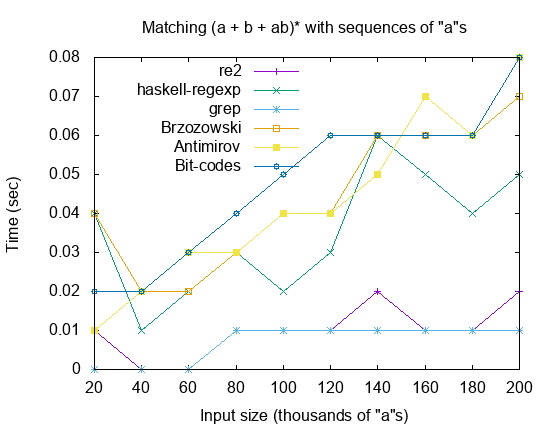
\includegraphics[width=0.45\textwidth]{as.png}
   \centering
   \caption{Results of experiment 1.}
   \label{fig:graph1}
\end{figure}

\begin{figure}[!ht]
    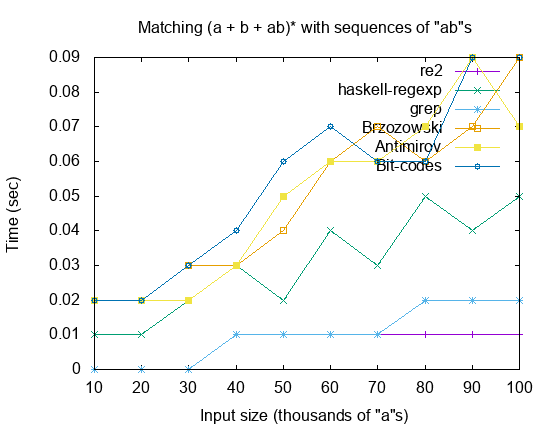
\includegraphics[width=0.45\textwidth]{abs.png}
   \centering
   \caption{Results of experiment 2.}
   \label{fig:graph2}
\end{figure}


Our tool behaves poorly when compared with all other options
considered. The cause of this inefficiency needs further
investigation, since the algorithm formalized uses POSIX 
disambiguation strategy, which avoid quotienting the result of derivative
operations w.r.t. ACUI axioms, as usual Brzozowski derivatives. We leave 
the proof that the formalized algorithm indeed produces POSIX parse trees 
for future work.

\section{Related Work}\label{sec:related}

\paragraph{Parsing with derivatives} Recently, derivative-based
parsing has received a lot of attention. Owens et al. were the first
to present a functional encoding of RE derivatives and use it to
parsing and DFA building. They use derivatives to build scanner
generators for ML and Scheme~\cite{Owens2009}; no formal proof of
correctness was presented.

Might et al.~\cite{Might2011} report on
the use of derivatives for parsing not only RLs but also context-free
ones. He uses derivatives to handle context-free grammars (CFG) and
develops an equational theory for compaction that allows for efficient
CFG parsing using derivatives. Implementation of derivatives for CFGs
are described by using the Racket programming
language~\cite{Felleisen2013}. However, Might et al. do not present
formal proofs related to the use of derivatives for CFGs.

Fischer et al.~describe an algorithm for RE-based parsing based on
weighted automata in Haskell~\cite{Fischer2010}.  The paper describes
the design evolution of such algorithm as a dialog between three
persons. Their implementation has a competitive performance when
compared with Google's RE library~\cite{re2}. This work also does not
consider formal proofs of RE parsing.

An algorithm for POSIX RE parsing is described
in~\cite{SulzmannL14}. The main idea of the article is to adapt
derivative parsing to construct parse trees incrementally to solve
both matching and submatching for REs. In order to improve the
efficiency of the proposed algorithm, Sulzmann et al. use a bit
encoded representation of RE parse trees. Textual proofs of
correctness of the proposed algorithm are presented in an appendix.

\paragraph{Certified parsing algorithms}. Certified algorithms for
parsing also received attention recently. Firsov et al.~describe a
certified algorithm for RE parsing by converting an input RE to an
equivalent NFA represented as a boolean matrix~\cite{FirsovU13}. A
matrix library based on some ``block'' operations~\cite{MacedoO13} is
developed and used Agda formalization of NFA-based parsing
{Norell2009}. Compared to our work, a NFA-based formalization requires
a lot more infrastructure (such as a Matrix library). No experiments
with the certified algorithm were reported.

Firsov describes an Agda formalization of a parsing algorithm that
deals with any CFG (CYK algorithm)~\cite{Firsov2014}. Bernardy
et al.~describe a formalization of another CFG parsing algorithm in
Agda~\cite{BernardyJ16}: Valiant's algorithm~\cite{Valiant1975}, which
reduces CFG parsing to boolean matrix multiplication. In both works,
no experiment with formalized parsing algorithms were reported.

A certified LR(1) CFG validator is described
in~\cite{Jourdan2012}. The formalized checking procedure verifies if
CFG and an automaton match. They proved soundness and completeness of
the validator in the Coq proof
assistant~\cite{Bertot2010}. Termination of the LR(1) automaton
interpreter is ensured by imposing a natural number bound on
allowed recursive calls.

Formalization of a parser combinator library was the subject of
Danielsson's work~\cite{Danielsson2010}. He built a library of parser
combinators using coinduction and provide correctness proofs of such
combinators.

Almeida et al.~\cite{AlmeidaMPS10} describe a Coq formalization of
partial derivatives and its equivalence with automata. Partial
derivatives were introduced by Antimirov~\cite{Antimirov91} as an
alternative to Brzozowski derivatives, since it avoids quotient
resulting REs with respect to ACUI axioms. Almeida et al. motivation
is to use such formalization as a basis for a decision procedure for
RE equivalence.

Ridge~\cite{Ridge2011} describes a formalization, in the HOL4 theorem
prover, of a combinator parsing library. A parser generator for such
combinators is described and a proof that generated parsers are sound
and complete is presented.  According to Ridge, preliminary results
shows that parsers built using his generator are faster than those
created by Happy parser generator~\cite{Happy}.

Ausaf et. al.~\cite{AusafDU16} describe a formalization, in
Isabelle/HOL~\cite{Nipkow02}, of the POSIX matching algorithm proposed
by Sulzmann et.al.~\cite{SulzmannL14}. They give a constructive
characterization of what a POSIX matching is and prove that such
matching is unique for a given RE and string. No experiments with the
verified algorithm are reported.


\section{Conclusion}\label{sec:conclusion}

We have given a complete formalization of a Bit-coded derivative-based 
parsing for REs in Agda. To the best of our knowledge, this is the first work
that presents a complete certification and that uses the certified
program to build a tool for RE-based search.

The formalized algorithm has 381 lines of code, organized in 2
modules. We have proven 18 theorems and lemmas to complete the
development. Most of them are immediate pattern matching functions
over inductive datatypes and were omitted from this text for brevity.
The verigrep tool has 3 parsing algorithms formalized in 1526 lines of code, 
distributed in 22 modules.

As future work, we intend to continue the development of verigrep by
certifying greedy and POSIX disambiguation strategies and finite state machine
based algorithms for parsing RE.

% \section*{References}
\bibliographystyle{ACM-Reference-Format}
\bibliography{main}

\end{document}

\end{document}
